% !TEX root = ../MasterThesis_Onoe.tex
% 上記はただのコメントではなく親ファイルの場所を教えているので
% 消してしまうとファイルごとのタイプセットができなくなるので注意。
% 親ファイル名を変更したときはここも変更する。

\chapter{序論} \label{sec:Intruduction}
本章では、はじめに1.1節で素粒子とそれらに働く相互作用を説明する標準模型(The Standard Model; SM)について述べる。そして1.2節にて将来の電子陽電子ヒッグスファクトリーである、国際リニアコライダー計画(International Linear Collider; ILC)の概要に触れたのち、1.3節でILCが探索する物理について、特にヒッグス粒子に関係した事項を中心に述べる。ILCの実現において必要なILCの検出器について1.4節で、ソフトウェアについて1.5節でまとめたのち、1.6節で本研究の目的を述べる。
\section{素粒子物理学}
\subsection{標準模型}
素粒子とは、物質を構成している究極要素をさす名称である。そして素粒子物理学は、それら構成要素とその間に働く相互作用の性質を解明する学問である。現代の素粒子物理学では、すべての現象を説明するための基本的な枠組みとして図\ref{sm}のような標準模型を掲げており、これは現時点の実験データと高い精度で一致することが確認されている。\\
\begin{figure}[ht]
	\begin{center}
 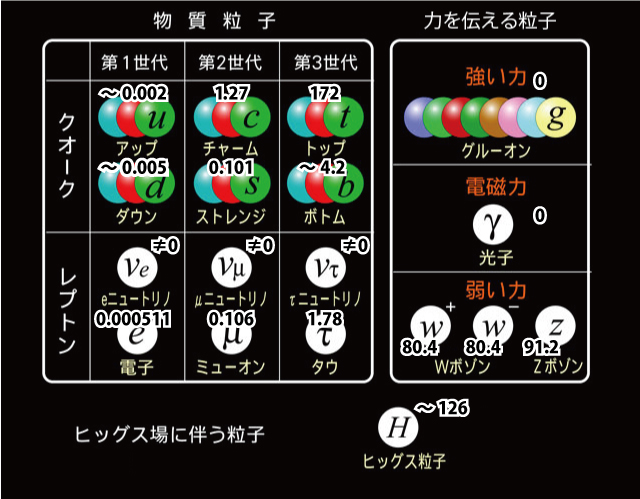
\includegraphics[keepaspectratio, scale=0.4]
 	{Figure/Introduction/sm.jpg}
 		\caption{素粒子の標準模型(数値は質量[$\mathrm{GeV/c^2}$])}
 		\label{sm}
	\end{center}
\end{figure}
 標準模型は、主に次に挙げる2つの基本的な前提に沿って記述されている。1つ目に、物質の究極要素である素粒子はクォークとレプトンというスピン1/2のフェルミオンである。2つ目に、素粒子の相互作用はゲージ理論によって記述され、標準模型における相互作用は電磁相互作用・弱い相互作用・強い相互作用の3つである。

物質の化学的性質を失わない最小単位は分子であり、分子はさらに原子の組み合わせによって構成されている。そして原子は原子核と電子によって構成されており、原子核は陽子と中性子のような核子からなっている。この核子を構成するものがクォークであり、標準模型においては6種類存在する。一方で、電子のような強い相互作用をしないものをレプトンと呼び、同様に6種類存在する。クォーク・レプトンともに3つの世代と2つの電荷タイプをもっており、世代の大きい粒子ほど重いため弱い相互作用により小さい世代のクォーク・レプトンへと崩壊する。

場の量子論では量子場$\phi$が素粒子と関連して記述されており、ラグランジアンによって相互作用の性質が記述される。ラグランジアンが量子場の局所的なゲージ対称性のもとで不変であると仮定すると、ゲージ場と呼ばれるベクトル場が現れるが、このゲージ場と量子場の積によって相互作用を表す理論をゲージ理論という。ゲージ粒子はこのゲージ場が粒子として現れたもので、素粒子の相互作用を媒介するとされているスピン1のゲージ粒子には、グルーオン・光子・$W$ボソン・$Z$ボソンの4種類がある。クォークとグルーオンの相互作用である強い相互作用は、量子色力学に基づき$SU(3)$対称性をもつ。また荷電粒子と光子の相互作用である電磁相互作用と$W$・$Z$ボソンを介する弱い相互作用は、グラショウ=ワインバーグ=サラム理論(GWS理論)\cite{gws}によって統一され電弱相互作用と呼ばれており、$SU(2)\times U(1)$対称性をもつ。これに加えて重力相互作用が存在するが、他の3つの相互作用と比較して非常に弱いため標準模型では扱われない。

本論文のテーマである電子・陽電子はレプトンに分類される素粒子であり、粒子・反粒子の関係にある。反粒子とはある粒子と符号の異なる電荷を持つが、質量やスピン角運動量など電荷以外は同じ特性を持つ粒子を指しており、陽電子は電子の反粒子である。粒子・反粒子の関係にある粒子はその質量エネルギーを放出して対消滅を起こす性質があり、ヒッグスファクトリーにおいてもこの現象によって別の素粒子を生成する。

また、標準模型は実験データと高い精度で一致しているが、標準模型だけでは説明しきれない物理も数多く存在しており、標準理論を越えた新しい物理(Beyond the Standard Model; BSM)を検証する実験が世界中で行われている。

\subsection{ヒッグス機構}
GWS理論においてゲージ粒子はゲージ対称性により質量項が禁止されているが、先述の$W$・$Z$ボソンはそれぞれ$\SI{80.4}{GeV/c^2}$、$\SI{91.2}{GeV/c^2}$の質量を持っている。標準模型ではこれを説明するためにヒッグス機構を導入し、ゲージ対称性が自発的に破れることで質量を獲得している。このヒッグス機構によると、宇宙の膨張によって真空は冷却されてヒッグスが凝縮した状態に相転移が起き、この相転移によって対称性が破れる。そのため真空に複素2次元のスカラー場としてヒッグス場$\Phi$を導入し、これとゲージ場との相互作用によって質量を持つとしている。またヒッグス場の存在と同時に、対応する粒子としてヒッグス粒子の存在が必要となる。ヒッグス場のポテンシャル\cite{gaugehiggs}は
\begin{align}
V(\phi) = {\mu}^2({\Phi}^\dag \Phi) + \lambda ({\Phi}^\dag \Phi)^2 (ただし{\mu}^2 < 0)
\end{align}
%ポテンシャルは正であるため自己結合定数$\lambda > 0$であり、
と書くことができ、ポテンシャルの概形は図\ref{higgspotential}のような形状になる。
\begin{figure}[H]
	\begin{center}
 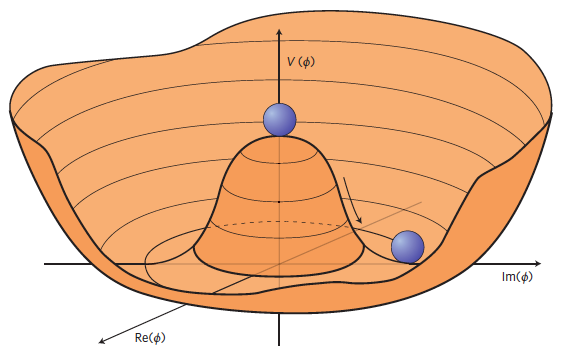
\includegraphics[keepaspectratio, scale=0.3]
 	{Figure/Introduction/higgspotential.png}
 		\caption{ヒッグスポテンシャル\cite{higgspotential}}
 		\label{higgspotential}
	\end{center}
\end{figure}

図\ref{higgspotential}のようなポテンシャルでは、$\mathrm{V(\phi)}$軸周りに真空がリング状に縮退している。また真空のポテンシャルは最小値をとる点で安定するが、ヒッグスポテンシャルにおいては一つの点をとると位相回転対称性が破れてしまう。このときヒッグス場に、
\begin{align}
\label{higgsvalue}
\langle \Phi \rangle = \frac{v}{2} = \sqrt{\frac{-{\mu}^2}{2\lambda}}
\end{align}
の有限の真空期待値が現れる。これによってゲージ粒子が質量を獲得する。より直感的には、真空に凝縮されたヒッグス場の中でゲージ粒子を加速しようとした時に、ヒッグス場から抵抗を受ける。この抵抗は、ゲージ場が1個のヒッグス粒子と衝突する頻度を意味する結合定数と、真空のヒッグスの密度に比例することから、質量は加速されにくさを表す量と考えることができる。

このヒッグス粒子は、2012年7月に欧州原子核研究機構 (Conseil Europ\'een pour la Recherche Nucl\'eaire; CERN) の大型ハドロン衝突型加速器(Large Hadron Collider; LHC)におけるATLAS、CMS実験によって発見され、理論と実験との一致が確認された。本論文のテーマであるヒッグスファクトリーでは、このヒッグス粒子を大量に生成し詳細に研究することを最大の目的としている。\\

\section{国際リニアコライダー計画; ILC}
国際リニアコライダー(International Linear Collider; ILC)は、東北地方北上山地が有力な建設候補地となっている電子陽電子衝突型線形加速器であり、将来のヒッグスファクトリーとしての稼働を期待されている。全長$\SI{20}{km}$の線形加速器を用いて電子と陽電子を加速し、中央のInteraction Point(IP)で衝突させることで様々な粒子を生成し、これを解析することでヒッグス粒子を始めとする新物理を探索することを目的としている(図\ref{ilc})。またILCは重心系エネルギー$\sqrt{s} = \SI{250}{GeV}$での運転開始を予定しているが、線形加速部を延長することで$\SI{1}{TeV}$を超えるエネルギーまでのアップグレードも可能になっており、各エネルギーにおける物理プログラムのメインターゲットは次のようになっている。
\begin{itemize}
\item $\sqrt{s} = \SI{250}{GeV}$:$Zh$随伴生成過程の研究
\item $\sqrt{s} = \SI{350}{GeV}$:$t\bar{t}$対生成、$WW$融合過程によるヒッグス生成
\item $\sqrt{s} = \SI{500}{GeV}$:ヒッグスの自己結合とトップ湯川結合の測定、高統計によるヒッグス精密測定
\item $\sqrt{s} = \SI{1}{TeV}$:ヒッグスの自己結合とトップ湯川結合の精密測定
\end{itemize}
\begin{figure}[t]
	\begin{center}
 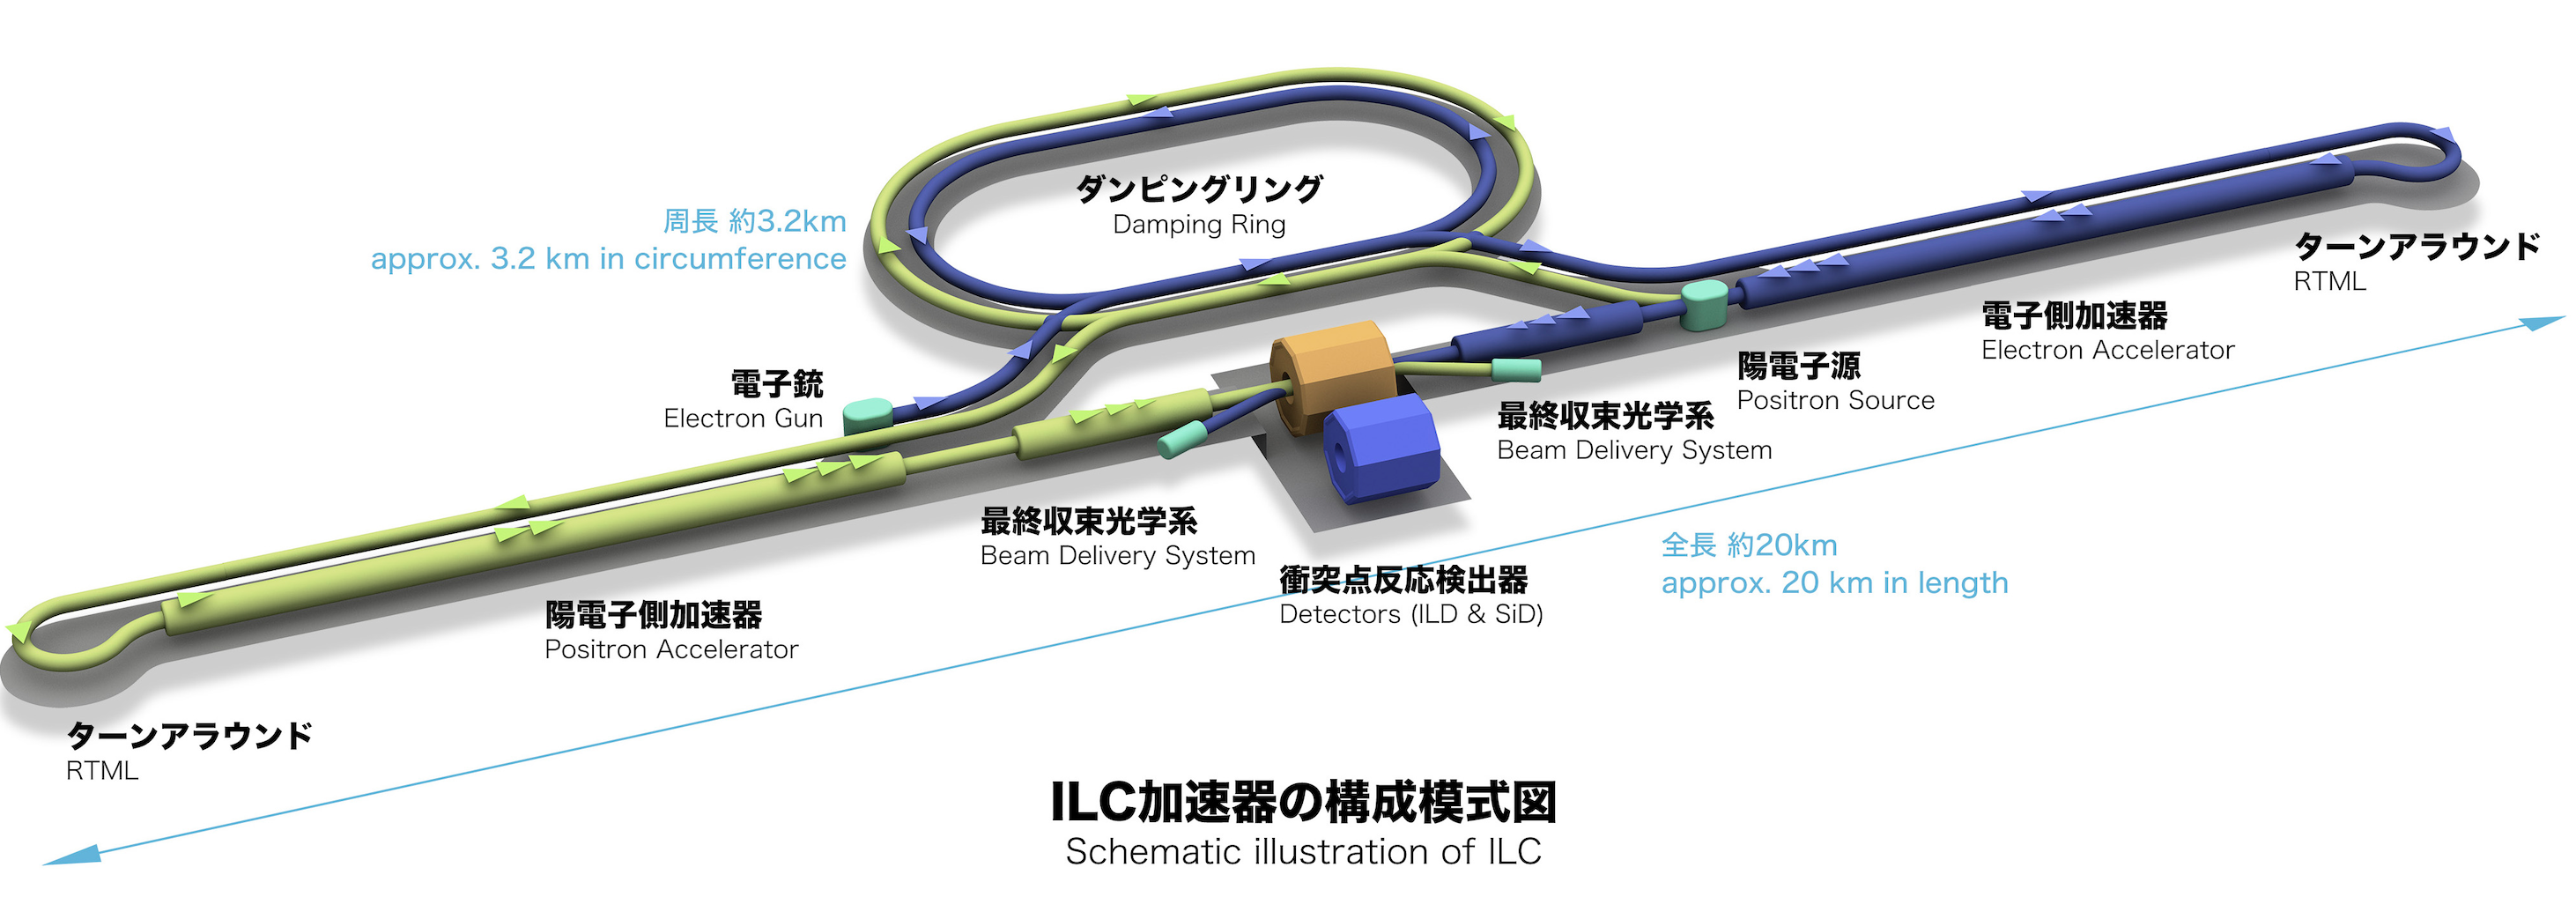
\includegraphics[keepaspectratio, scale=0.25]
 	{Figure/Introduction/ilc.png}
 		\caption{ILCの概略図}
 		\label{ilc}
	\end{center}
\end{figure}

ヒッグス粒子を発見したLHCと比較してILCには以下の4つの利点が存在する。1つ目はLHCが複合粒子であるハドロンのコライダーであるのに対して、ILCはレプトンコライダーである点である。ILCでは背景事象が少ないクリーンな環境で、ヒッグス粒子を始めとした網羅的な新物理探索が可能になっている。また、LHCでは断面積を計算する上でQCDに基づく系統的な不確定性が存在するが、ILCでは電弱相互作用のみについて考えることができるため、高精度な理論検証が可能になる。2つ目は加速粒子である電子陽電子が粒子反粒子の関係にある点である。粒子反粒子が対消滅することで全エネルギーを目的粒子の生成に効率的に用いることができる。加えてILCのビームはバンチ構造をしており、全事象を記録したデータをバンチの衝突間隔を利用して転送し、オフラインで事象選択を行うことができるためトリガーレスで運転することが可能である。これによって、多重度が低く運動量が小さい軌跡だけを持つ事象のような、トリガーで捉えることが難しい事象までをも活かすことができる。3つ目はビーム起因のバックグラウンドが小さい点である。これによって崩壊点検出器をビームからおよそ\SI{15}{mm}と近い距離におくことができ、フレーバーの識別において$b$フレーバのみでなく$c$フレーバの識別も可能となる。4つ目はビーム偏極が全エネルギーで可能となっている点である。ビーム偏極とは進行方向に対するスピンを意味しており、これによって測定可能な物理量を増やすことができる。
\section{ILCの物理}
\subsection{ヒッグス生成過程と質量精密測定}
1.1節で述べた通り、ILCはヒッグスファクトリーとしての役割を期待されている。ヒッグスファクトリーでは、ヒッグス粒子を大量に生成し崩壊過程を精密測定することで、他の粒子との結合定数を測定し標準模型を検証することができる。ILCにおけるヒッグス粒子の生成断面積は図\ref{hcs}のようになっており、運転開始で予定している$\sqrt{s}=\SI{250}{GeV}$付近では、主に$Zh$随伴生成過程の断面積が最大となる。この$Zh$随伴生成過程では、反跳粒子である$Z$ボソンを正確に再構成することで、ヒッグス粒子の質量を
\begin{align}
\label{recoil}
M_{recoil}^2 = {( \sqrt{s} - E_{ff} )}^2 - {|\vec{p}_{\ ff}|}^2
\end{align}
によって、高い精度で求めることができる。($E_{ff}$は$Z$ボソンが崩壊するフェルミオン対のエネルギーを、$\vec{p}_{\ ff}$は運動量を表す。)

LHCのような複合粒子同士の衝突では、始状態の運動量が定まっていないことに加えバックグラウンドとなる事象も多い。しかしILCの反応過程では、始状態の運動量がわかっているため、反跳粒子を正確に再構成することでヒッグス粒子の崩壊モードに依存せず全断面積の測定が可能となっている。このようヒッグス粒子の崩壊モードに依存しない測定によってヒッグス粒子のinvisibleな崩壊の存在を検証することが出来る。これにはヒッグス粒子が暗黒物質や後述する超対称性粒子に崩壊するモードなどが含まれており、標準模型を超える新物理の検証を行うことが可能である。

\begin{figure}[h]
\begin{center}
 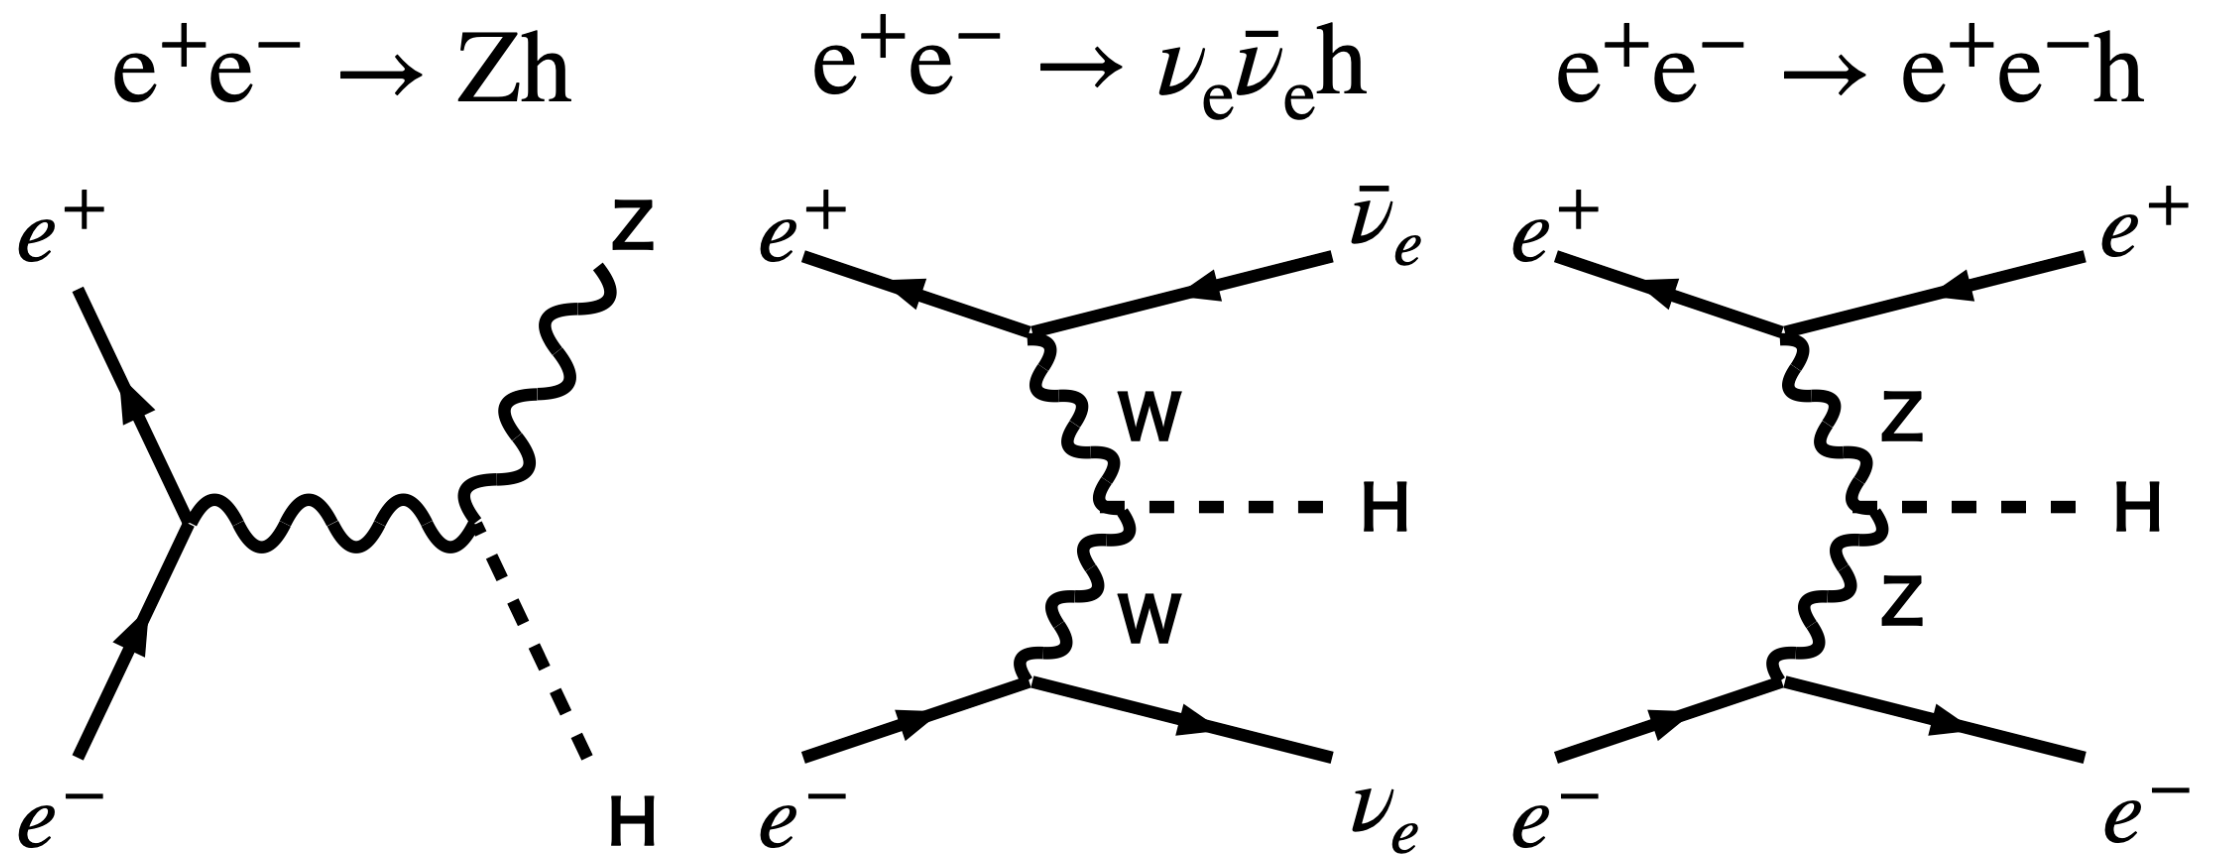
\includegraphics[keepaspectratio, scale=0.18]
 	{Figure/Introduction/higgs_cs_feynman.png}
	\caption{$Zh$随伴生成、$WW$融合反応、$ZZ$ 融合反応におけるファインマンダイアグラム\cite{tdr2}。}
\end{center}
\end{figure}

\begin{figure}[H]
	\begin{center}
 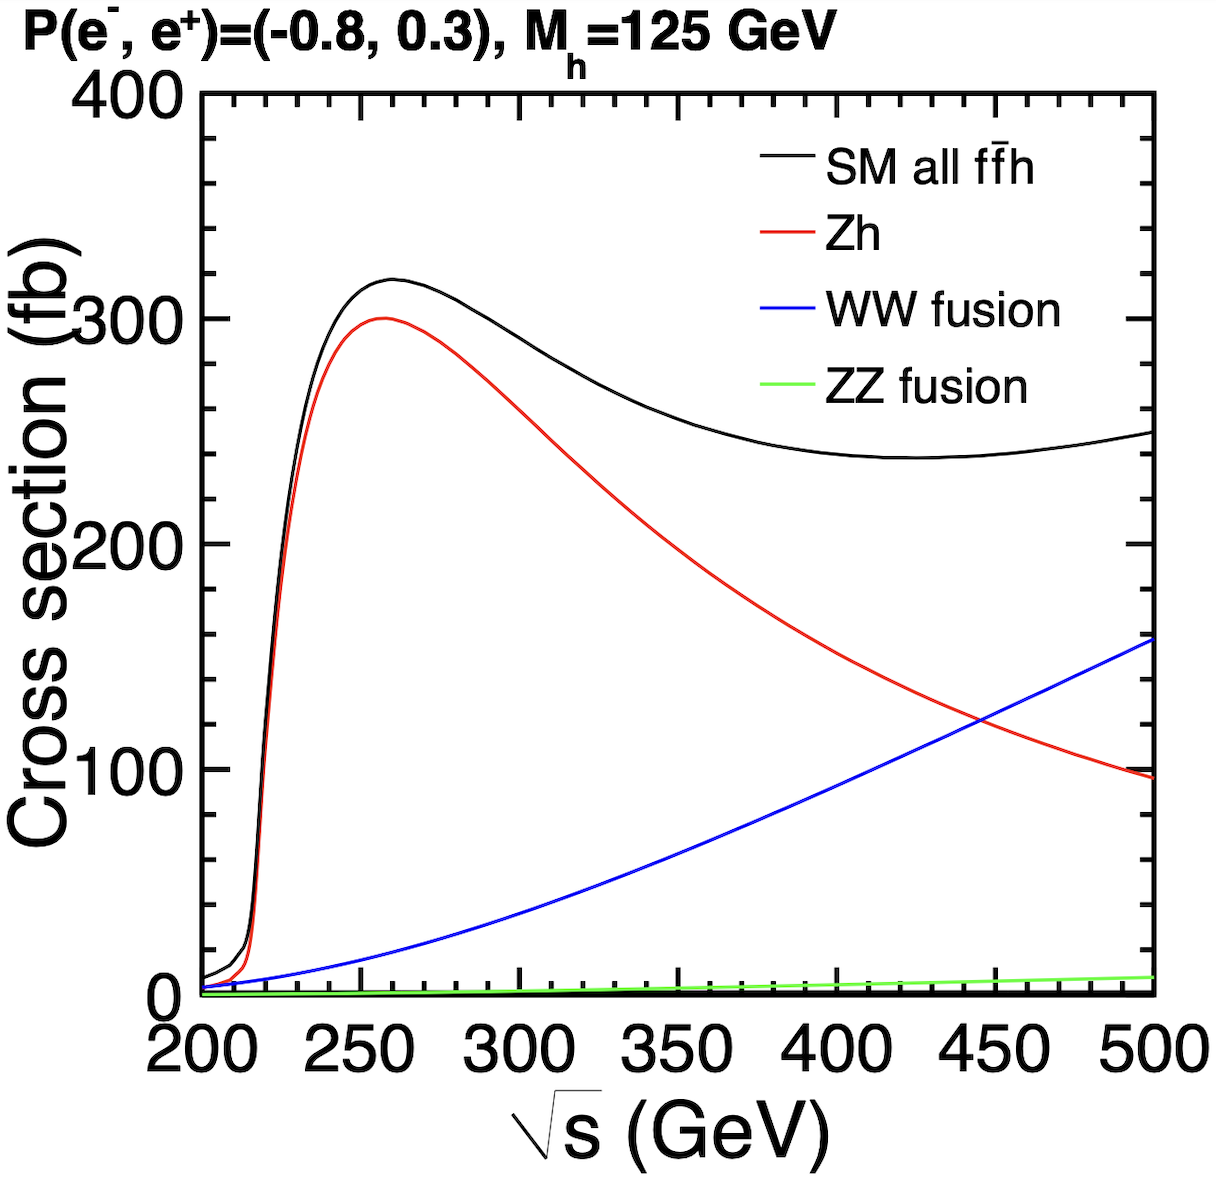
\includegraphics[keepaspectratio, scale=0.2]
 	{Figure/Introduction/hcs.png}
	 	\caption{ILCの重心系エネルギーに対するヒッグス生成断面積。ヒッグス粒子の質量が$m_h=\SI{125}{GeV}$であるとして、$Zh$随伴生成、$WW$融合反応、$ZZ$融合反応をそれぞれ赤、青、緑線で示している\cite{tdr2}。}
 	\label{hcs}
	\end{center}
 \end{figure}
 
\subsection{ヒッグス結合定数の精密測定}
電子陽電子衝突によって生成されるヒッグス粒子は不安定であるため、より質量の小さい粒子のペアに崩壊する。標準模型におけるヒッグス粒子の各質量に対する崩壊分岐比の割合を図\ref{higgs_decay}に、$m_h = \SI{125}{GeV}$ における崩壊分岐比を表\ref{HiggsDecayonILC}示す。ILCではヒッグス粒子の生成断面積と全崩壊幅を精密に測定することができるため、ヒッグス粒子の崩壊分岐比を精密に決定することができる。この崩壊分岐比はヒッグス粒子の結合定数の2乗に比例しており、標準模型を超える新物理のシナリオにおいてヒッグス粒子の結合定数に生じるズレを検証することができる。
\begin{figure}[H]
 \begin{minipage}[h]{.45\linewidth}
	\begin{center}
 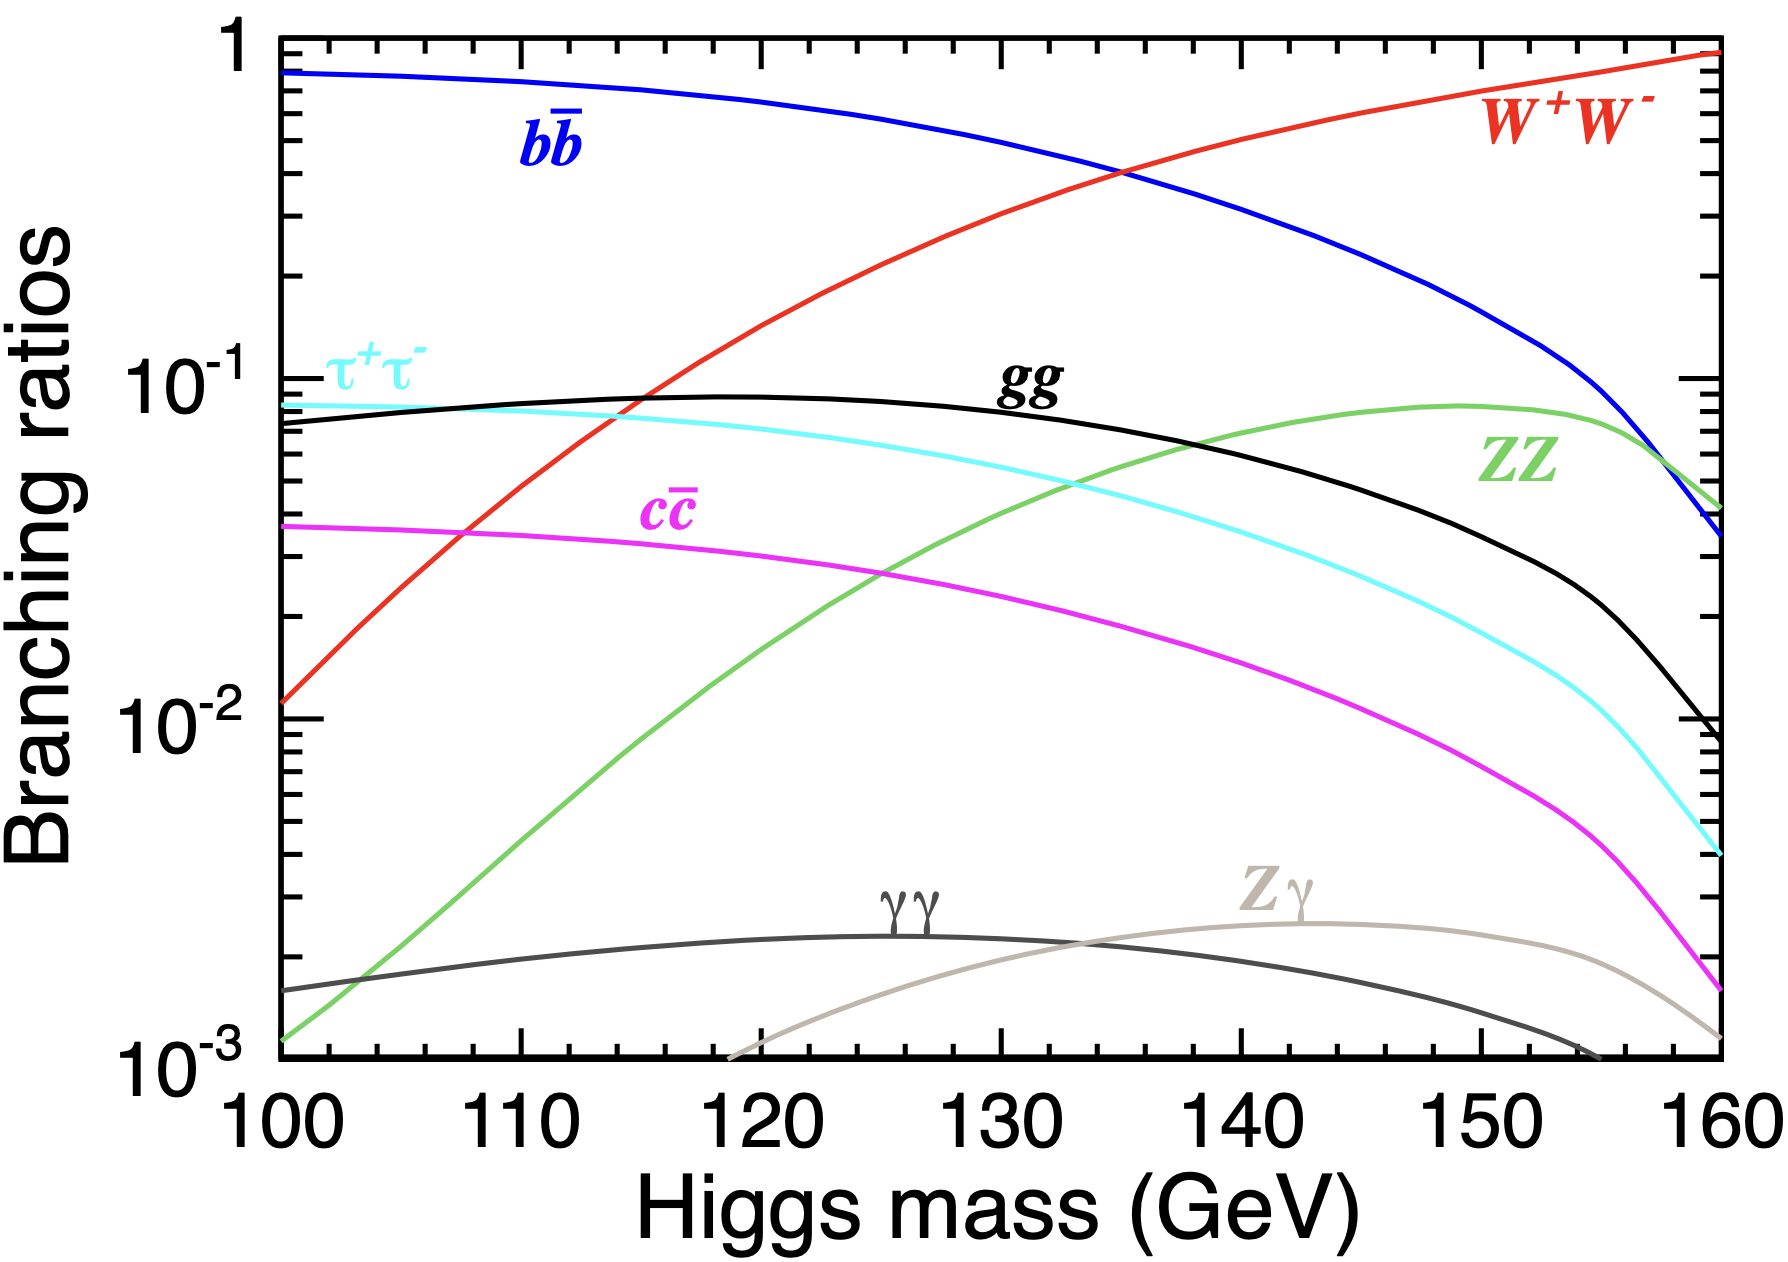
\includegraphics[keepaspectratio, scale=0.2]
 	{Figure/Introduction/higgs_decay.png}
 	\caption{標準模型におけるヒッグス粒子の質量と崩壊分岐比の関係}
 	\label{higgs_decay}
	\end{center}
 \end{minipage}
 \hfill
% ----- 表: ヒッグス崩壊分岐比 ------
\begin{minipage}[ht]{.45\linewidth}
%\def\@captype{table}
 \centering
  \begin{tabular}{clc}
   \hline
   崩壊モード & 崩壊分岐比\\
   \hline \hline
   $b\bar{b}$ & 58.1\, \%\\
   $WW$ & 21.5\, \%\\
   $gg$ & 8.2\, \%\\
   ${\tau}^+ {\tau}^-$ & 6.3\, \%\\
   $c \bar{c}$ & 2.9\, \%\\
   $ZZ$ & 2.6\, \%\\
   $\gamma \gamma$ & 0.2\, \%\\
   \hline
  \end{tabular}
  \tblcaption{$m_h = \SI{125}{GeV}$におけるSMヒッグス粒子の崩壊分岐比}
  \label{HiggsDecayonILC}
 \end{minipage}
 \end{figure}
% --------------------

以下では、結合定数の精密測定によって検証可能な新物理について述べる。図\ref{bsmdecay}は新物理の各シナリオにおける、標準模型ヒッグス粒子との結合定数のズレを表す。
\begin{itemize}
\item{超対称性理論}

超対称性理論(Supersymmetry; SUSY)は、フェルミオンとボソンを交換する変換に対する不変性(超対称性)を定義する理論である。この理論においては、標準模型におけるすべての粒子に対してスピンが1/2異なる超対称性パートナーが導入される。超対称性が完全である場合、標準模型粒子と同じ相互作用を持ち、電弱スケールでは超対称性の破れによって$\mathrm{TeV}$スケールの質量を持つ必要性があるが、現段階ではSUSY粒子は発見に至っていない。SUSYでは図\ref{bsmdecay}のように主にヒッグス粒子する$b$クォーク・$\tau$レプトンとの結合が大きくなる。
\item{複合ヒッグス模型}

ヒッグス粒子はTeVスケールにおいて複合粒子のように振る舞い、その内部により基本的な粒子を持っているとするモデルが複合ヒッグス模型である。この模型ではCompositeness scaleによって抑制される高次の作用素により、標準模型と比べて結合定数が大きくずれてしまう。Compositeness scaleを$f$とすると、ヒッグス粒子のゲージボソンやフェルミオンへの結合は、
\begin{align}
\frac{g_{hxx}}{g_{h_{SM}xx}} \simeq 1 \pm \mathcal{O}(v^2 / f^2)
\end{align}
のオーダーで表される。図\ref{bsmdecay}において複合ヒッグス模型では、標準模型に比べて粒子との結合が小さくなっている。
\end{itemize}
\begin{figure}[H]
	\begin{center}
 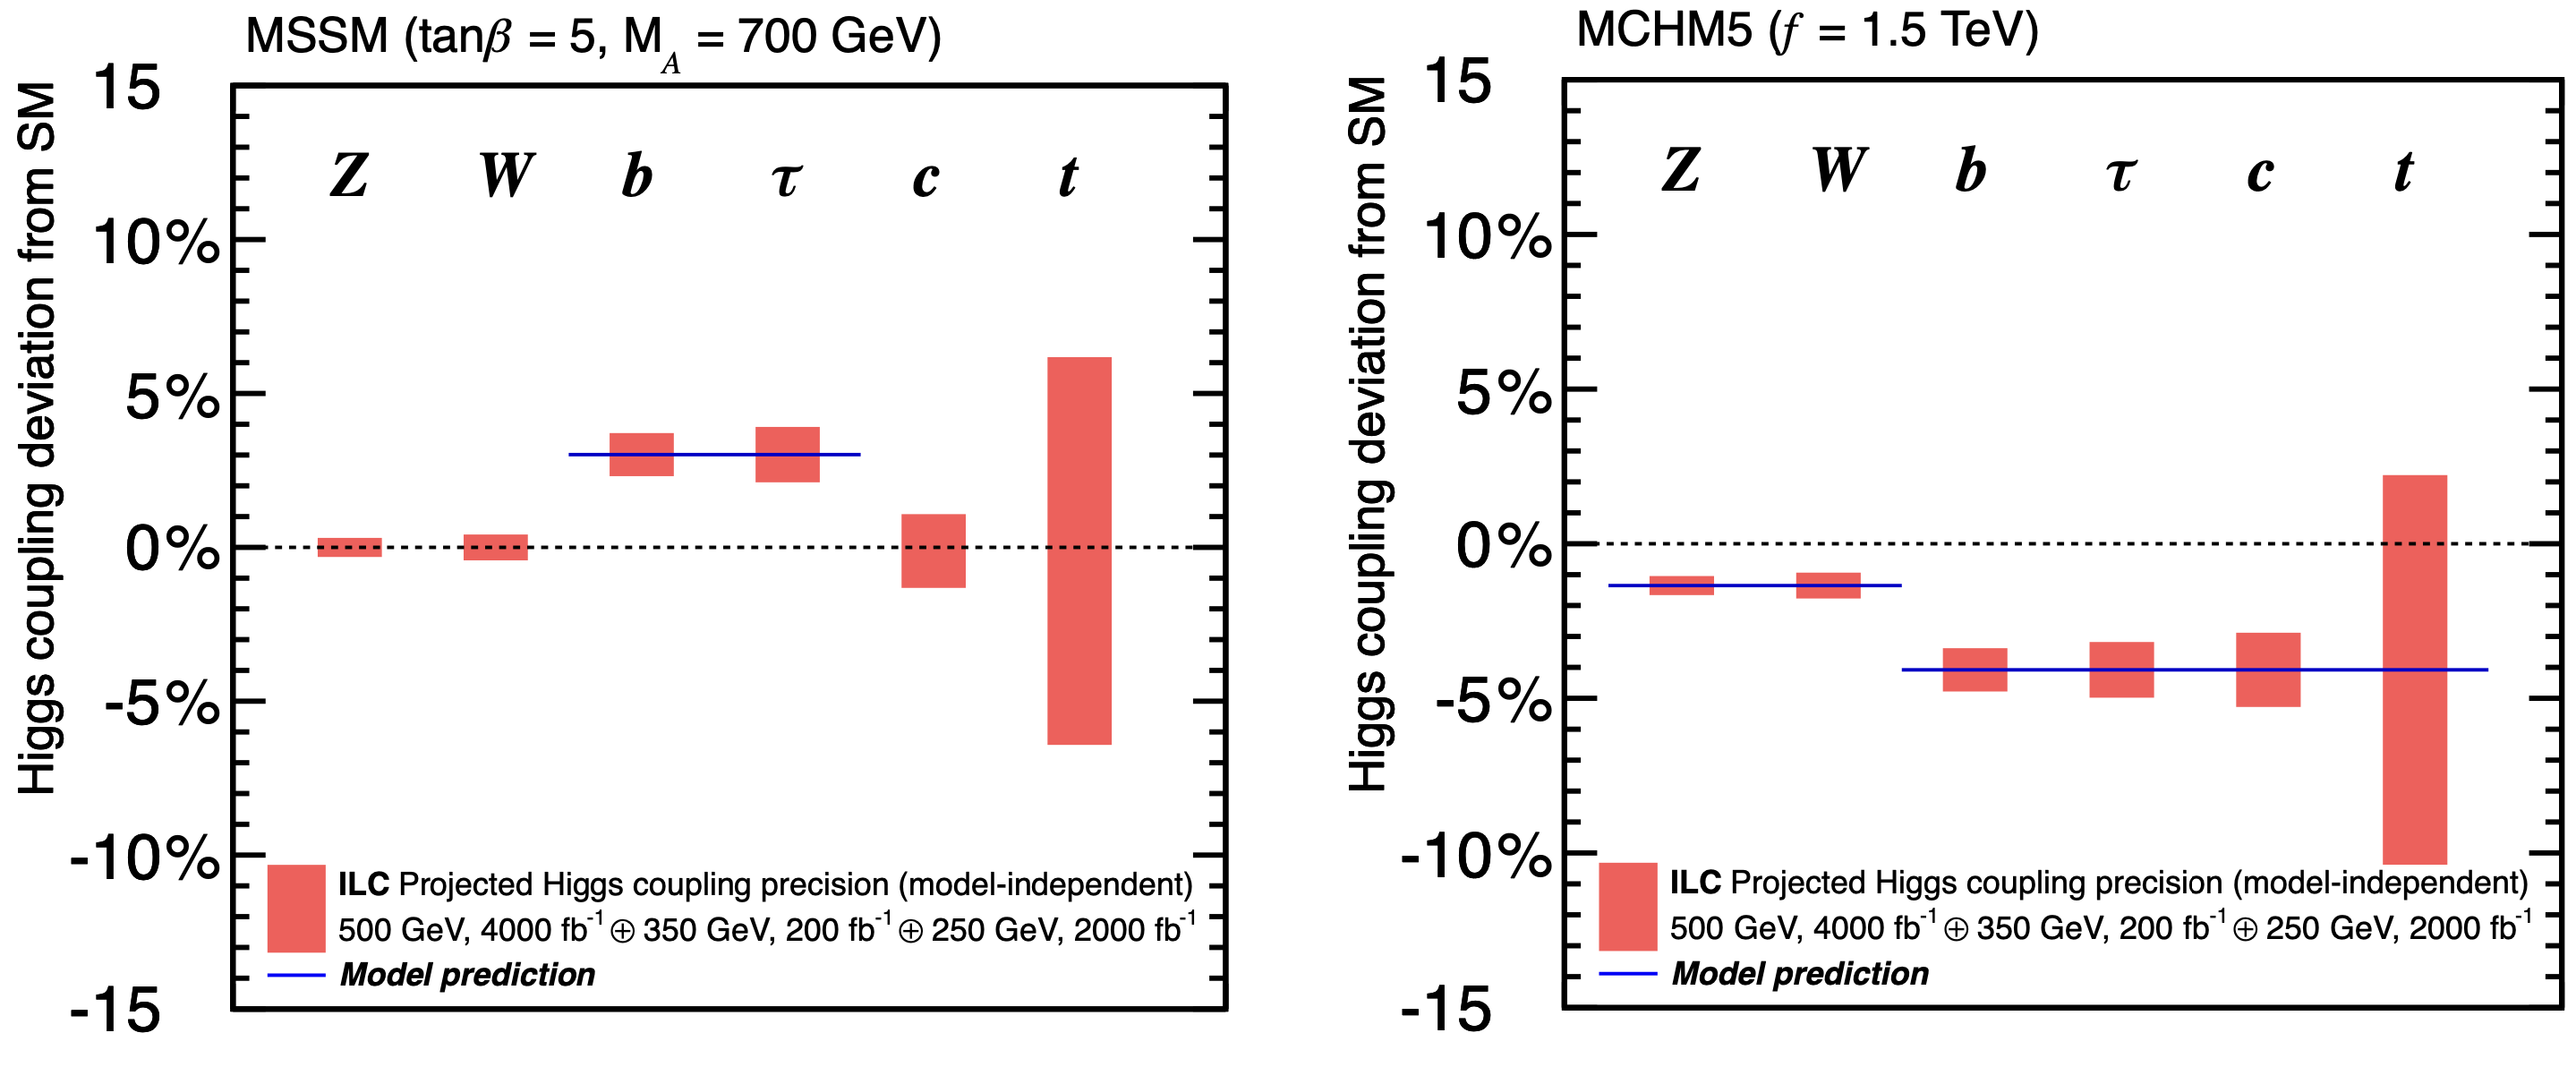
\includegraphics[keepaspectratio, scale=0.25]
 	{Figure/Introduction/bsmdecay.png}
 		\caption{2つの新物理のモデルにおける、標準模型のヒッグス粒子結合定数とのずれ。 (左) 超対称性 (SUSY) モデル (右) 複合ヒッグスモデル。誤差棒は1\, $\sigma$の範囲を表している。}
 		\label{bsmdecay}
	\end{center}
\end{figure}
 ヒッグスの崩壊分岐比の測定精度は信号事象数をS、背景事象数をNとするとS/$\mathrm{\sqrt{S+N}}$となり、背景事象の影響を十分低減させることができた場合には不定性を1\%以下まで下げることができる。図\ref{lhcvsilc}ではLHCとILCにおけるヒッグス粒子の結合定数の測定精度を表しており、ILCではLHCに比べておよそ1桁優れた精度で測定することができる。これを達成するために、高い検出器性能と精度の高い事象再構成・解析手法が求められている。
\begin{figure}[H]
	\begin{center}
 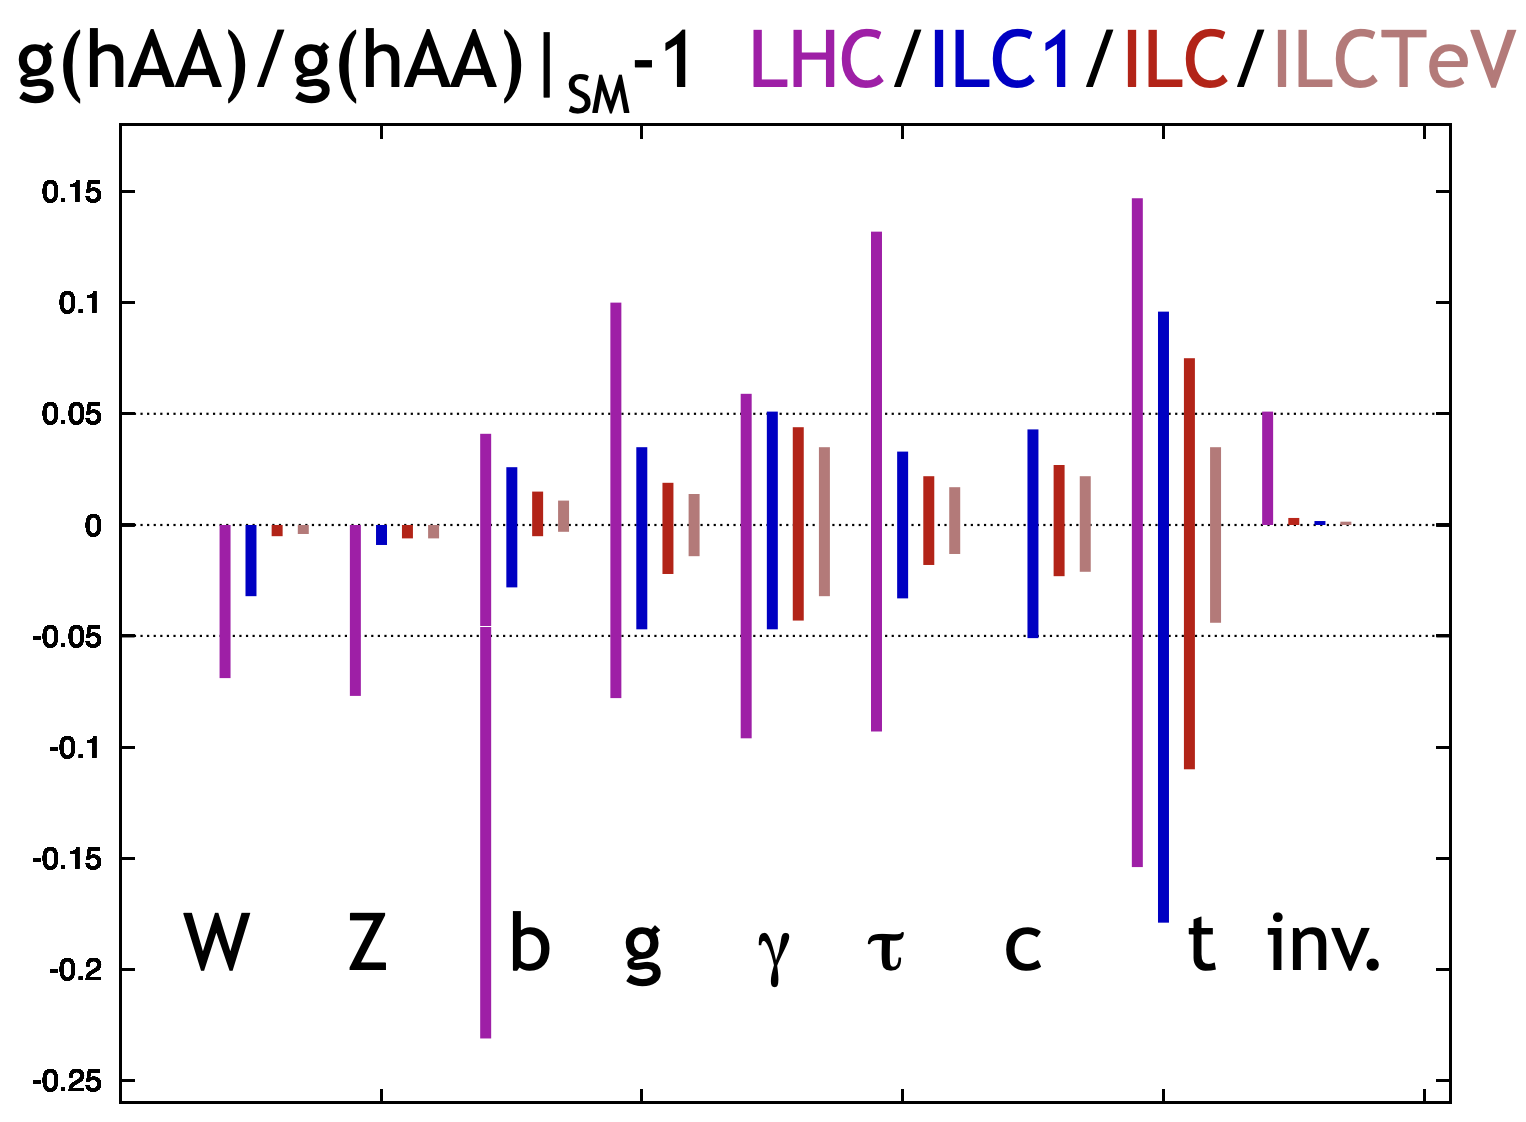
\includegraphics[keepaspectratio, scale=0.3]
 	{Figure/Introduction/lhcvsilc.png}
 		\caption{ILCとHL-LHCにおけるヒッグス粒子の各粒子に対する結合定数の測定精度予測。誤差棒は1$\sigma$の範囲を表している。(紫:LHC ($300 \mathrm{fb^{-1}}$), 青:ILC1 ($\SI{250}{GeV}$) , 臙脂:ILC ($\SI{500}{GeV}$) , 薄橙:ILCTeV ($\SI{1}{TeV}$))\cite{decaybsm}}
 		\label{lhcvsilc}
	\end{center}
\end{figure}

\subsection{ヒッグス自己結合}
$\SI{500}{GeV}$以上のILCでは図\ref{selfcoupling}のような、$e^+e^- \rightarrow Zhh$反応の断面積を測定することで、自己結合について探索することができる。ゲージ不変性によりヒッグスの三点結合は、四点結合における真空凝縮としてのみ起こることができるため、三点結合を確認することでヒッグス場の真空凝縮について検証することができる。ILC$\SI{500}{GeV}$における図\ref{selfcoupling}の断面積は$\SI{0.2}{fb}$と小さく高統計を得ることが難しいため、崩壊$e^+e^- \rightarrow Zhh \rightarrow q\bar{q}bb\bar{b}\bar{b}$における$b$フレーバーの識別精度が非常に重要になる。
\begin{figure}[h]
	\begin{center}
 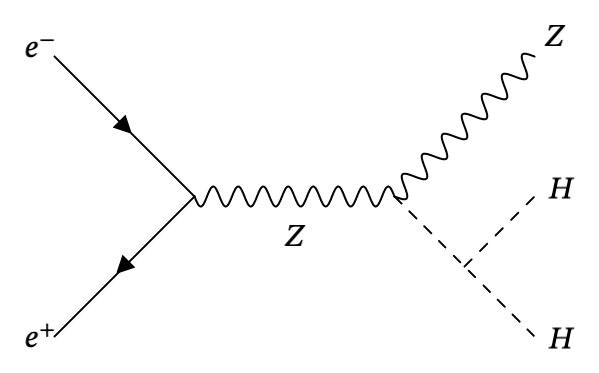
\includegraphics[keepaspectratio, scale=0.3]
 	{Figure/Introduction/selfcoupling.png}
 		\caption{ヒッグス自己結合$e^+e^- \rightarrow Zhh$}
 		\label{selfcoupling}
	\end{center}
\end{figure}
\subsection{階層性問題}
ヒッグス粒子の質量はLHCによって$\SI{125}{GeV/c^2}$と測定されている。しかしヒッグス粒子の質量は、図\ref{hierarchy}のような高次ダイアグラムからプランクスケール ($10^{19} \mathrm{GeV}$) 程度の質量補正を受けることが分かっている。そのため標準模型を超える新物理による質量の量子補正をキャンセルする解決策がなければ、量子補正を受ける前の質量がプランクスケール程度の質量であり、それに対して偶然プランクスケール程度の負の量子補正がかかって$\SI{125}{GeV/c^2}$の質量を再現しているということになってしまう(ファインチューニング)。これを回避するために、以下に挙げるようなTeVスケールの超対称性理論や余剰次元理論など新物理によるシナリオが提案されている。これらのシナリオにおけるヒッグス粒子との結合定数は標準模型における予測からズレることとなるため、ILCにおいてヒッグス粒子の精密測定を行うことで崩壊分岐比を決定することの意義は大きいと言える。
\begin{figure}[h]
	\begin{center}
 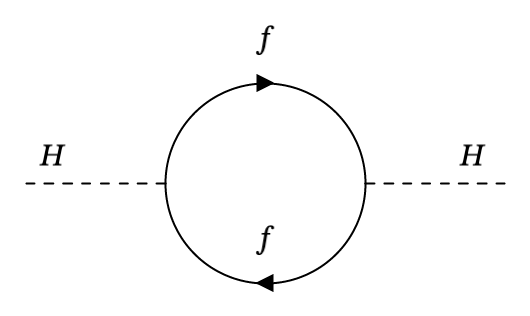
\includegraphics[keepaspectratio, scale=0.3]
 	{Figure/Introduction/feynman.png}
 		\caption{ヒッグス粒子の質量補正となるフェルミオンループ}
 		\label{hierarchy}
	\end{center}
\end{figure}
\begin{itemize}
\item{超対称性理論}\\
階層性問題においては、超対称性によりヒッグス粒子の質量補正に関する2次の発散をフェルミオンの寄与で打ち消す。これによって、対数による発散に落とすことができる。
\item{余剰次元理論}\\
余剰次元理論とは、四次元時空以外にも次元があるとする理論である。この理論では空間の次元数を増やすことで、増えた次元のゲージ場にヒッグス場の起源を求める。この場合にはゲージ不変性により、繰り込みの発散が現れないため階層性問題に対応できる。
\end{itemize}
\subsection{その他の新物理}
上にあげた階層性問題に関する物理に加え、トップクォークの質量の精密測定、電弱相互作用の精密検証が可能であり、ILCの実現やそのアップグレードを通して宇宙の謎に迫る大発見を期待できる。
\section{ILCの検出器}
ILC の検出器(図 \ref{ilcdetector} )には、日欧が中心となって開発が進められている International Large Detector(ILD)と、米国が中心となって開発が進められている Silicon Detector (SiD) の二つのコンセプトが提案されており、ILC ではこれら2つの検出器が IP を共有できるように push-pull 方式を採用する予定である。またILD、SiDともにParicle Flow Algorithm(PFA)という事象再構成アルゴリズムに沿って最適化されている。
\begin{figure}[h]
	\begin{center}
        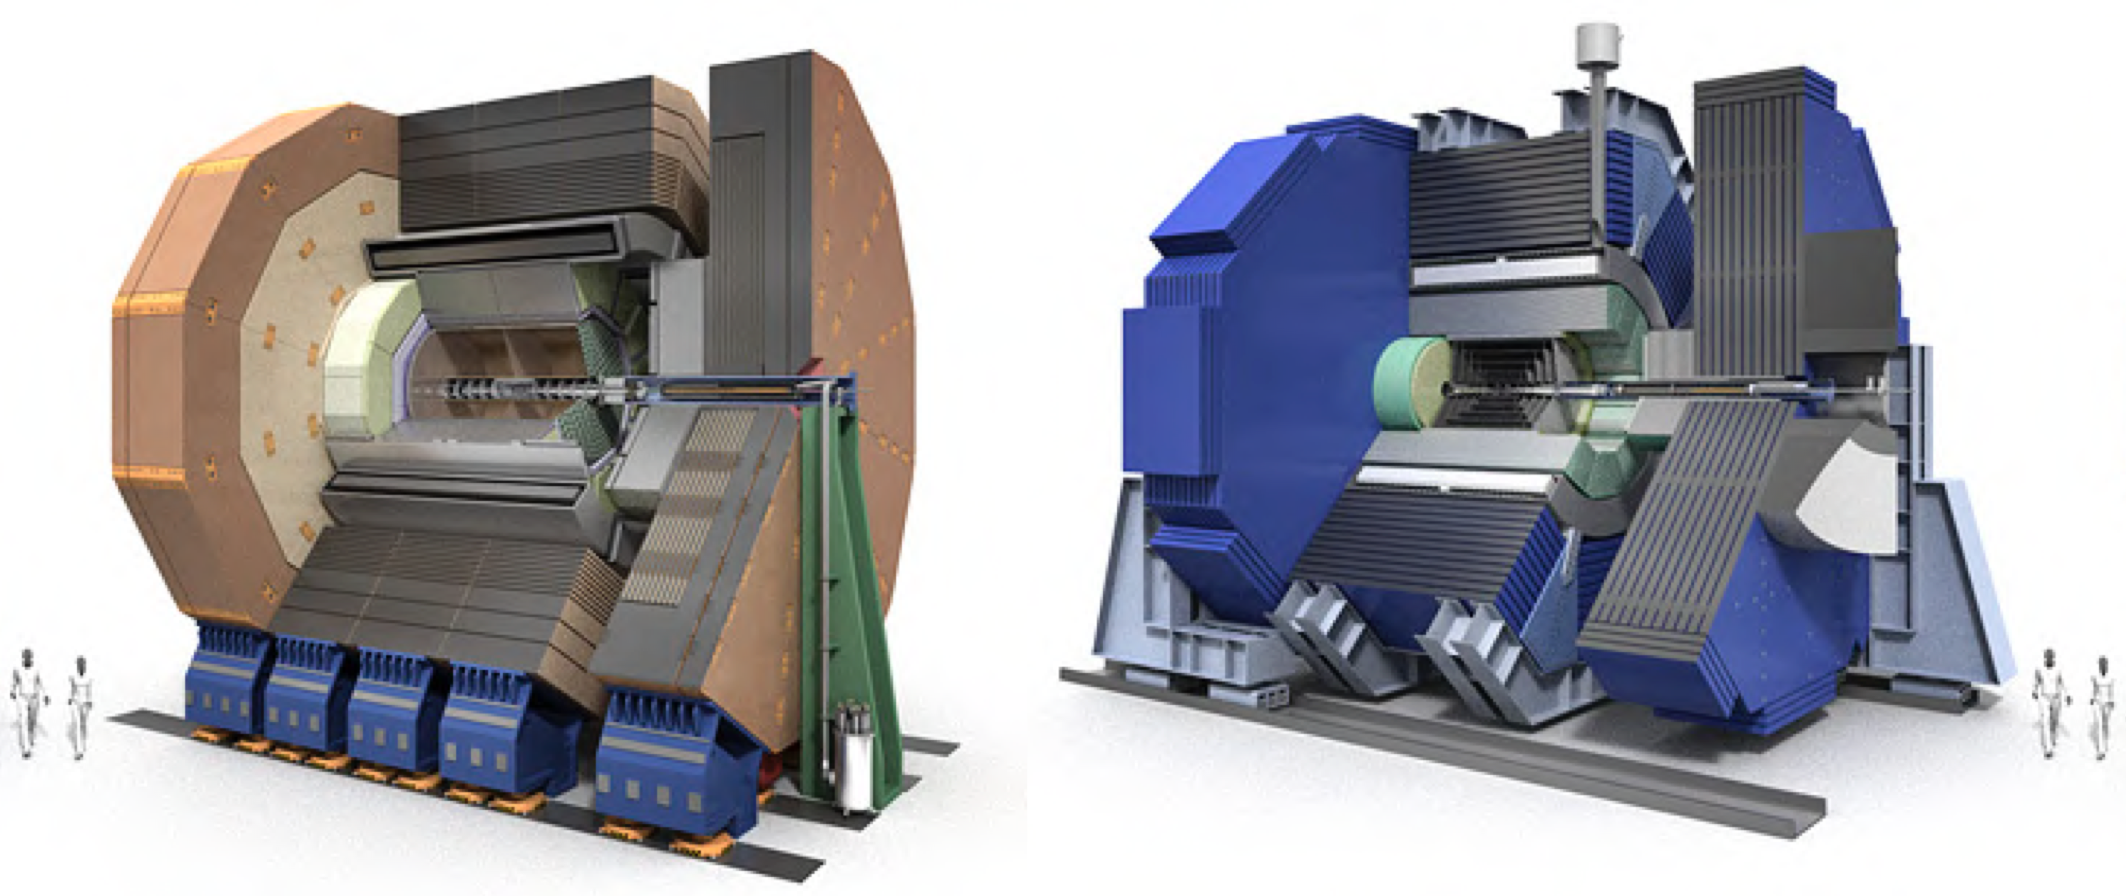
\includegraphics[keepaspectratio, scale=0.4]
 	{Figure/Introduction/detector.png}
 		\caption[ILDとSiDの全体図]{(左) ILD (右) SiD の全体図\cite{tdr2}}
 		\label{ilcdetector}
	\end{center}
\end{figure}
\subsection{ILDで検出器可能な粒子群}
ILCの電子陽電子衝突で生じる粒子は、ヒッグス粒子などの重いボソンを介した後に、クォークやグルーオン、レプトン、光子に崩壊する。この中でもクォークとグルーオンはQCDにおける閉じ込めにより単体で存在することができず、クォーク対となって多数のハドロン(強い相互作用で結合した複合粒子)を発生させる。また、レプトンのうちニュートリノは物質とほとんど相互作用を起こさず、測定器を通り抜けてしまうため、直接検出することは出来ない。そのため実際に測定器で検出することができるのは、終状態としてハドロンが束になったハドロンジェット、レプトン、光子となる。
\subsection{Particle Flow Algorithm; PFA}
前節の通りILCで生成されるクォークやグルーオンは、ジェットの終状態として検出される。そのためILCの物理を探求する上で必要となる粒子識別や事象再構成において、ジェットのエネルギーは非常に重要な情報であり、一般的にジェットのエネルギー分解能は
\begin{align}
\frac{{\sigma}_E}{E} = \frac{a}{\sqrt{E}} \oplus \frac{b}{E} \oplus c
\end{align}
として表される。ここで、$a,b,c$を係数に$E$はエネルギーを、$\oplus$は2乗和を表しており、第一項はカロリメータに由来する統計項を、第二項は補正項、第三項は定数項となっている。従来の素粒子実験におけるエネルギー測定では、およそ7割に相当する粒子がハドロンカロリメータでエネルギーを測定されるが、ハドロンカロリメータはそれ以外の検出器と比較してエネルギー分解能が低く、およそ$\sigma_E/E=55\, \%/\sqrt{E(\mathrm{GeV})}$の分解能となっている。ILCではジェットエネルギー分解能$\sigma_E/E=30\, \%/\sqrt{E(\mathrm{GeV})}$を目指しており、これを達成するために導入されているアルゴリズムがParticle Flow Algorith\cite{pfa}である。PFAはジェット内の粒子をその種類ごとに最適な検出器でエネルギー測定を行うことでジェットエネルギー分解能を向上させる再構成手法であり、過去の実験結果から、ジェット中に含まれる主な粒子の種類の典型的な割合 ($Z \rightarrow q\bar{q}$の場合) とそれに対応する検出器について以下のように分かっている(表\ref{pfa})。
\begin{table}[h]
 \centering
  \begin{tabular}{clll}
   \hline
   粒子のタイプ & \cth{検出器} & \cth{ジェット中のエネルギー割合}\\
   \hline \hline
   荷電粒子 & \cth{飛跡検出器} &  \cth{62\%}\\
   光子 & \cth{ECAL} &  \cth{27\%}\\
   中性ハドロン & \cth{HCAL} &  \cth{10\%}\\
   ニュートリノ & \cth{-} &  \cth{1\%}\\
   \hline
  \end{tabular}
   \caption{ジェットを占める各粒子と対応する検出器}
   \label{pfa}
\end{table}

\subsection{International Large Detector: ILD}
ILD \cite{tdr2}は内側から順に崩壊点検出器、飛跡検出器、電磁カロリメータ、ハドロンカロリメータ、ミューオン検出器で構成されている。カロリメータとミューオン検出器の間には$3.5$テスラのソレノイドコイルが設置されている。図\ref{ild}に断面図を示す。
\begin{figure}[H]
	\begin{center}
 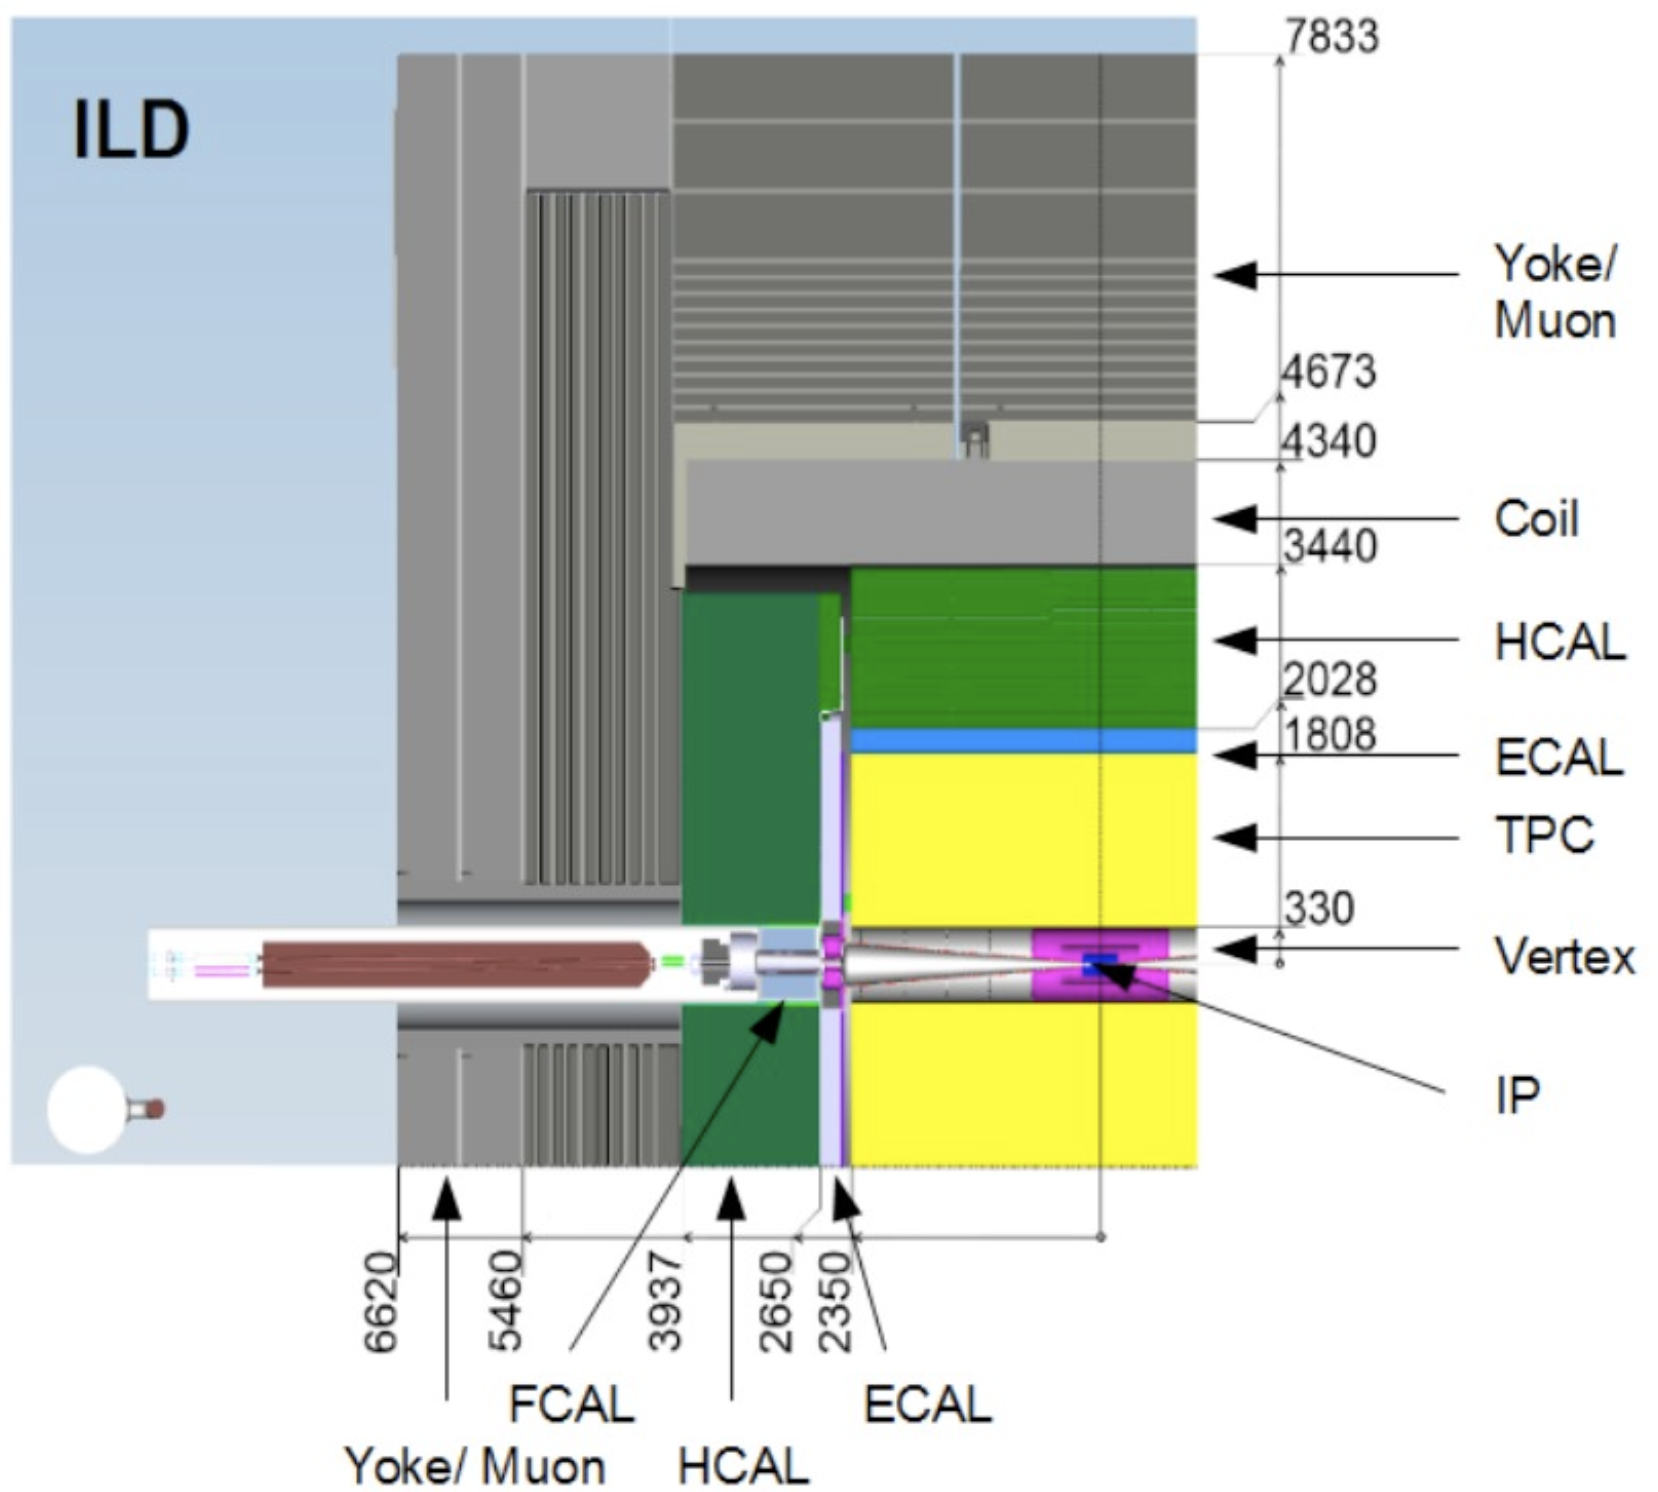
\includegraphics[keepaspectratio, scale=0.25]
 	{Figure/Introduction/ild.png}
 		\caption {ILDの断面図}
 		\label{ild}
	\end{center}
\end{figure}

\subsubsection{崩壊点検出器}
崩壊点検出器はIPに最も近い場所に置かれる検出器であり、図\ref{vertexdetector}のようにシリコンピクセルセンサーが両面に貼られた層をILDの半径方向に3層重ねた構造になっている。このシリコンピクセルセンサーで飛跡を高い位置分解能のもと検出することで、荷電粒子の生成点を高い精度で決定することが出来る。これによって短寿命粒子の崩壊点を高精度に再構成することができ、再構成された二次崩壊点はジェットのクォークフレーバーを識別する上で非常に重要な情報となる。ILCでは飛跡検出における位置分解能$\sigma$ (式\ref{resolution}) を目標としており、そのためにCMOSセンサー、DEPFET、Fine Pixel CCD、SOIなど様々な技術候補が研究されている\cite{tdr2}。
\begin{align}
\label{resolution}
\sigma [\mathrm{\mu m}] = 5 \oplus \frac{10} {p[\mathrm{GeV/c}] \ {\sin^{3/2}{\theta}}}
\end{align}
\begin{figure}[H]
	\begin{center}
 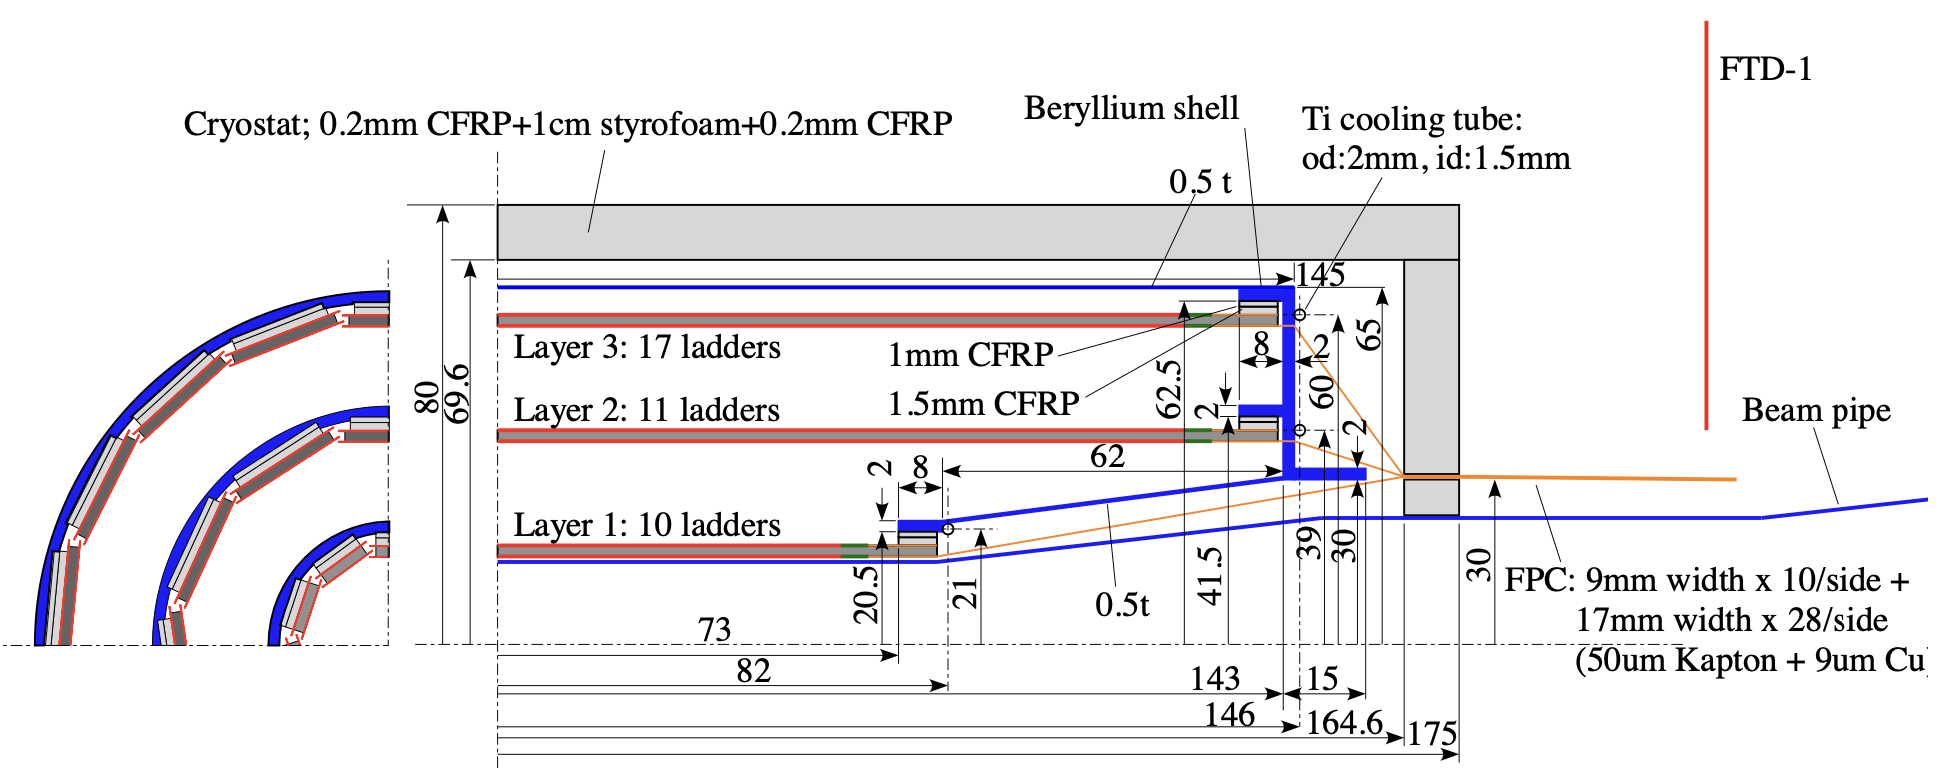
\includegraphics[keepaspectratio, scale=0.3]
 	{Figure/Introduction/vertexdetector.png}
 		\caption {ILD崩壊点検出器の構造}
 		\label{vertexdetector}
	\end{center}
\end{figure}
\subsubsection{中央飛跡検出器}
中央飛跡検出器は崩壊点検出器の外側に位置しており、Time Projection Chamber(TPC)とその周囲に設置されるシリコン検出器のハイブリッドで構成されている。TPCは大型のガスチェンバーであり、荷電粒子の通過でガス内に生じる電離電子を電極間にかけられた電場によってドリフトし、ドリフト時間などの情報をもとに飛跡を3次元的に再構成する検出器である。荷電粒子の飛跡を再構成することで運動量の測定が可能であり、粒子の検出数の多さから高い運動量分解能を持つ。さらに信号の大きさからエネルギー損失も測定することが可能であり、これは粒子識別において重要な役割を果たす。
\subsubsection{カロリメータ}
カロリメータは入射粒子のエネルギーを測定するための検出器で、ILDでは内側から電磁カロリメータ(ECAL)、ハドロンカロリメータ(HCAL)によって構成されており、またビーム軸方向に対して前方カロリメータ(FCAL)が設置される。これらILDのカロリメータにはサンプリング型カロリメータが提案されており、シャワーを起こすための吸収層と生成されたシャワー内の粒子のエネルギーを測定する検出層が交互に組み合わさった構造となっている。

ECALは主に電磁シャワー内の光子のエネルギーを測定するために利用される。ILDでは後述のPFAのためジェット内の粒子を分離できる高精細なカロリメータが必要とされており、吸収層には物質量が大きいため放射長が短く、モリエール半径の小さいタングステンが検討されている。また、検出層には読み出しセルが高精細なシリコン検出器を用いるシリコン電磁カロリメータ(SiECAL)やシンチレータストリップを用いるシンチレータカロリメータ(ScECAL)が提案されている。

HCALは荷電ハドロンと中性ハドロンのエネルギー損失を分離し、中性ハドロンのエネルギーを測定するための検出器である。HCALではハドロンとの相互作用を起こすための吸収層に鉄が用いられ、検出層には \SI{3}{cm}角のシンチレータタイルを用いてシンチレーション光を検出するアナログカロリメータ(AHCAL)と、ガラス抵抗板チェンバー (RPC) を用いて、$\SI{1}{cm}$角$2\mathrm{bit}$の信号を読み出すセミデジタルカロリメータ(SDHCAL)の2つが提案されている。

\subsubsection{ミューオン検出器}
ミューオン検出器はその名の通りミューオンを検出する検出器である。ミューオンは物質中で電磁シャワーやハドロンシャワーをほとんど生成しないため貫通力が大きく、IPから遠い検出器の最も外側に設置されており、RPCとSiPMシンチレータストリップの両方が検討されている。

\section{ILCのソフトウェア}
\subsection{イベントジェネレータと検出器シミュレーション}
ILCをはじめとする線型加速器には「iLCSoft」というソフトウェアフレームワークが開発されており、検出器シミュレーションから事象再構成までを実行することができる。iLCSoft内では専用のLCIOフォーマットを使用し、C++アプリケーションフレームワークであるMarlinによって運用され、検出器のジオメトリなどの記述にはDD4hepというツールキットを使用するという点で統一されている。

ILCは将来実験計画であるため、現在実験データは存在しないがシミュレーションによって検出器応答や新物理探索など研究が可能であり、本論文における研究で扱うデータもモンテカルロ(Monte Carlo; MC)法に基づくソフトウェア群を用いて生成したシミュレーションデータである。図\ref{ilcsoft}にILCにおけるソフトウェアの流れを示す。シミュレーションではまず、Whizardというイベントジェネレータを用いて、標準模型や様々な理論を背景とした物理事象を生成する。Wizardでは終状態で最大8粒子までの事象を生成し、Pythiaによって粒子の崩壊過程のシミュレーションを行う。更に生成されたイベントに対して、DDSimというGeant4をベースとした検出器シミュレーションを実行し、粒子から検出器ヒットデータが生成される。
\begin{figure}[h]
	\begin{center}
 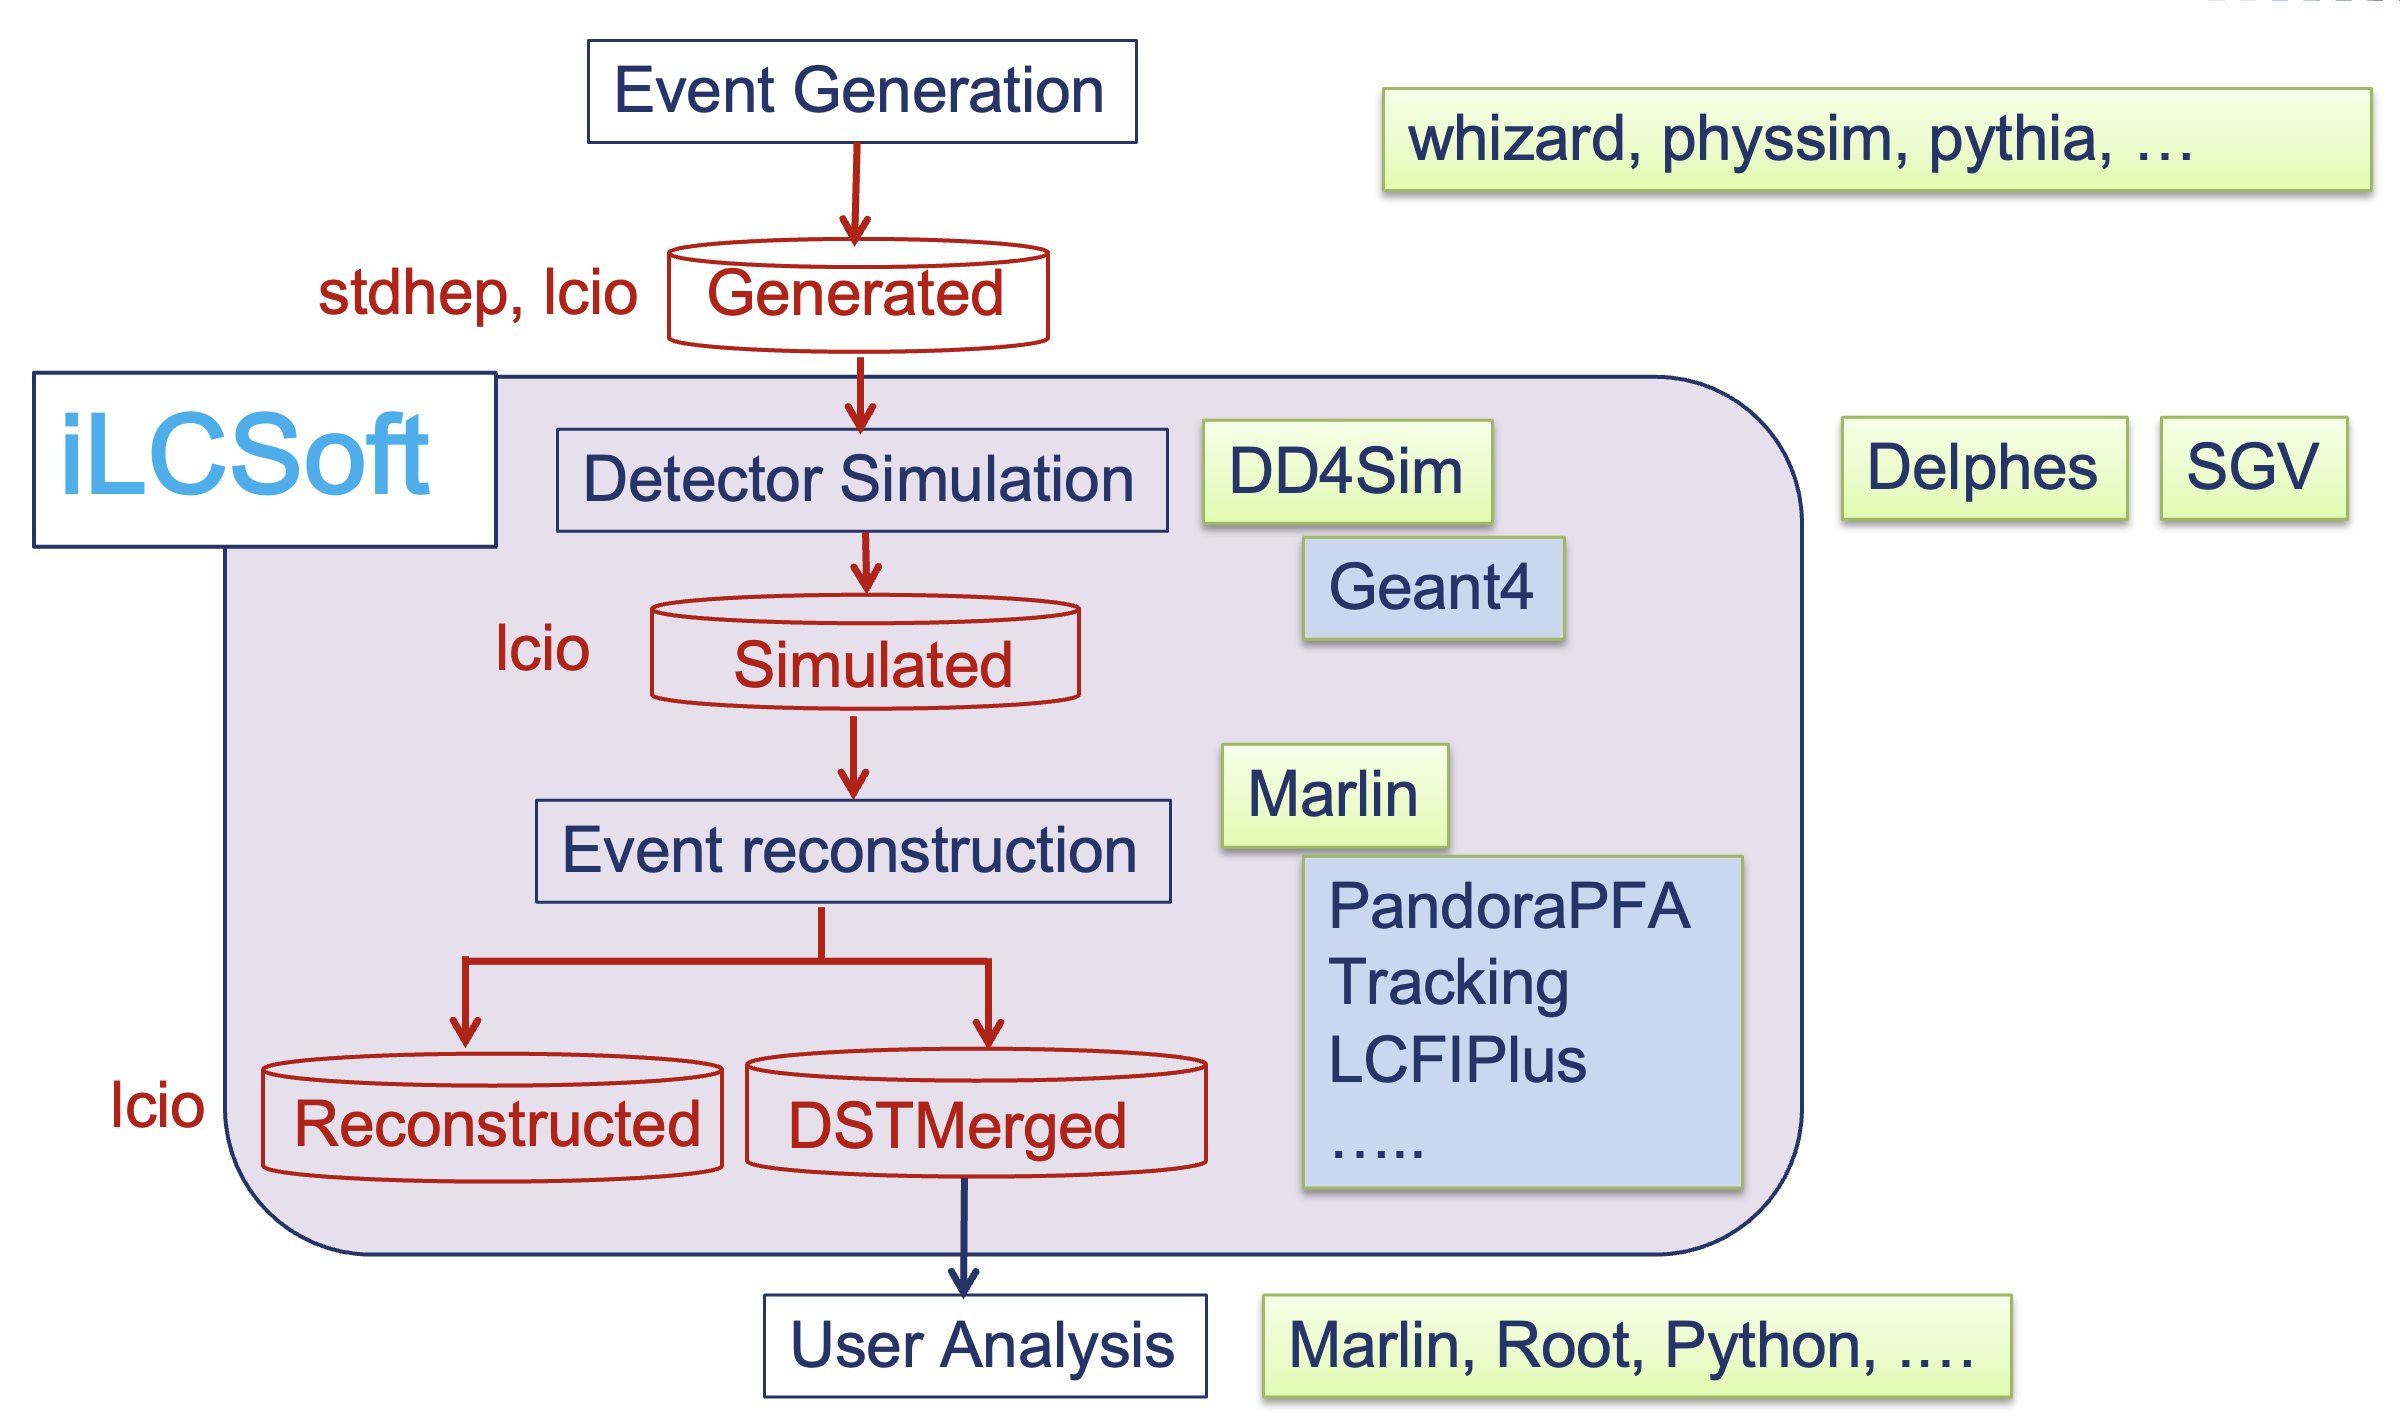
\includegraphics[keepaspectratio, scale=0.25]
 	{Figure/Introduction/ilcsoft.png}
 		\caption {ILCにおけるシミュレーションと事象再構成、物理解析の流れとソフトウェア}
 		\label{ilcsoft}
	\end{center}
\end{figure}

\subsection{事象再構成}
前節までで生成された検出器ヒットをもとに、終状態粒子のエネルギーや飛跡を推定する事象再構成が行われる。iLCSoftでは、Marlinによって測定器出力のデジタル化や飛跡再構成、PFAを行ったのちにジェットの再構成を実行し、物理解析へと繋げていく。iLCSoftにおいて、ジェットの再構成にあたる崩壊点検出からフレーバー識別のプロセスは、LCFIPlus~\cite{lcfiplus}というフレームワークで実行することができる。

\subsubsection{飛跡再構成}
多数の飛跡を含むジェットは各検出器を通過するため、検出器ヒットをもとにフィッティングを行うことで飛跡は再構成することができる。特に崩壊点検出器では主に飛跡の方向情報を、中央飛跡検出器では運動量や時間情報を取得し、様々なパターン認識アルゴリズムを有するMarlinTrkによって再構成される。荷電粒子の飛跡が再構成されたのち、PFAによって粒子の種類ごとのジェットエネルギーの再構成を行い、荷電粒子だけで中性粒子の情報も用いて以降のプロセスでジェットの再構成を行う。

\subsubsection{崩壊点検出}
ジェットはIPで生成された粒子が崩壊を繰り返し、多くの飛跡を残すことで再構成される。この粒子が崩壊する点を崩壊点(Vertex)と呼び、特にIPをprimary vertex、そこで生成された粒子の二次崩壊点をsecondary vertexと呼ぶ。LCFIPlusにおける崩壊点検出では、主に2本以上の飛跡の組み合わせから飛跡の発生源となる点を、${\chi}^2$値が最小値をとるフィッティングによって求める Vertex Fitter プロセスを用いる。この情報をもとに、primary vertexの再構成をtear-downアルゴリズムを用いて行う。tear-downアルゴリズムでは、全ての飛跡に対してIPを崩壊点とするフィッティングをVertex Fitterによって行い、一定の閾値に到達するまで${\chi}^2$値の大きい飛跡から排除していく。そしてprimary vertex に使用されていない全ての飛跡に対して再びフィッティングを行い、 ${\chi}^2$値や不変質量、運動量などを用いたカットや、飛跡同士の関係性の評価を行い、secondary vertexを再構成している。

\subsubsection{ジェットクラスタリング}
ILCの終状態の多くは4ジェット以上のマルチジェットであり、これらを幾つかのグループに分ける(クラスタリング)することでフレーバー識別の精度を向上させることができる。そのためジェットクラスタリングのプロセスでは、再構成された崩壊点やレプトンの情報をジェットのコアとし、Durham\cite{durham}のクラスタリングアルゴリズムを用いてクラスタリングを行う。具体的には、崩壊点やレプトンの特徴的な物理量や飛跡同士の開き角とエネルギーを用いて、全飛跡に対してクラスタリングを行う。

\subsubsection{フレーバー識別}
崩壊点の情報や飛跡の情報など20程度の物理量をもとに、多変量解析によってジェットの親粒子のフレーバー識別が行われる。LCFIPlusではROOT\cite{root}のTMVA\cite{tmva}パッケージを使用して、従来の機械学習手法であるBoosted Decision Trees(BDTs)を用いた識別が行われている。LCFIPlusでは$b$フレーバーのジェット、$c$フレーバーのジェット、u・d・sフレーバーのジェットの3つを分類している。分類においては、$b$・$c$フレーバーのハドロンは衝突点から離れたところで崩壊するという特徴がある。(図\ref{bcjets})ハドロンの寿命$\tau$は光速$c$を用いて、$b$ハドロンでおよそ$c\tau = 400 \sim \SI{500}{um}$、$c$ハドロンでおよそ$c\tau = 20 \sim \SI{300}{um}$である。上記に加えて$b$ハドロンから派生した$c$ハドロンも崩壊するため、1つのジェット中に崩壊点を2つもつ。これらの情報やジェットの物理量を用いてフレーバーを識別することができる。そのため崩壊点検出のプロセスにおいて、高精度に崩壊点を求めることが重要となる。
\begin{figure}[H]
	\begin{center}
 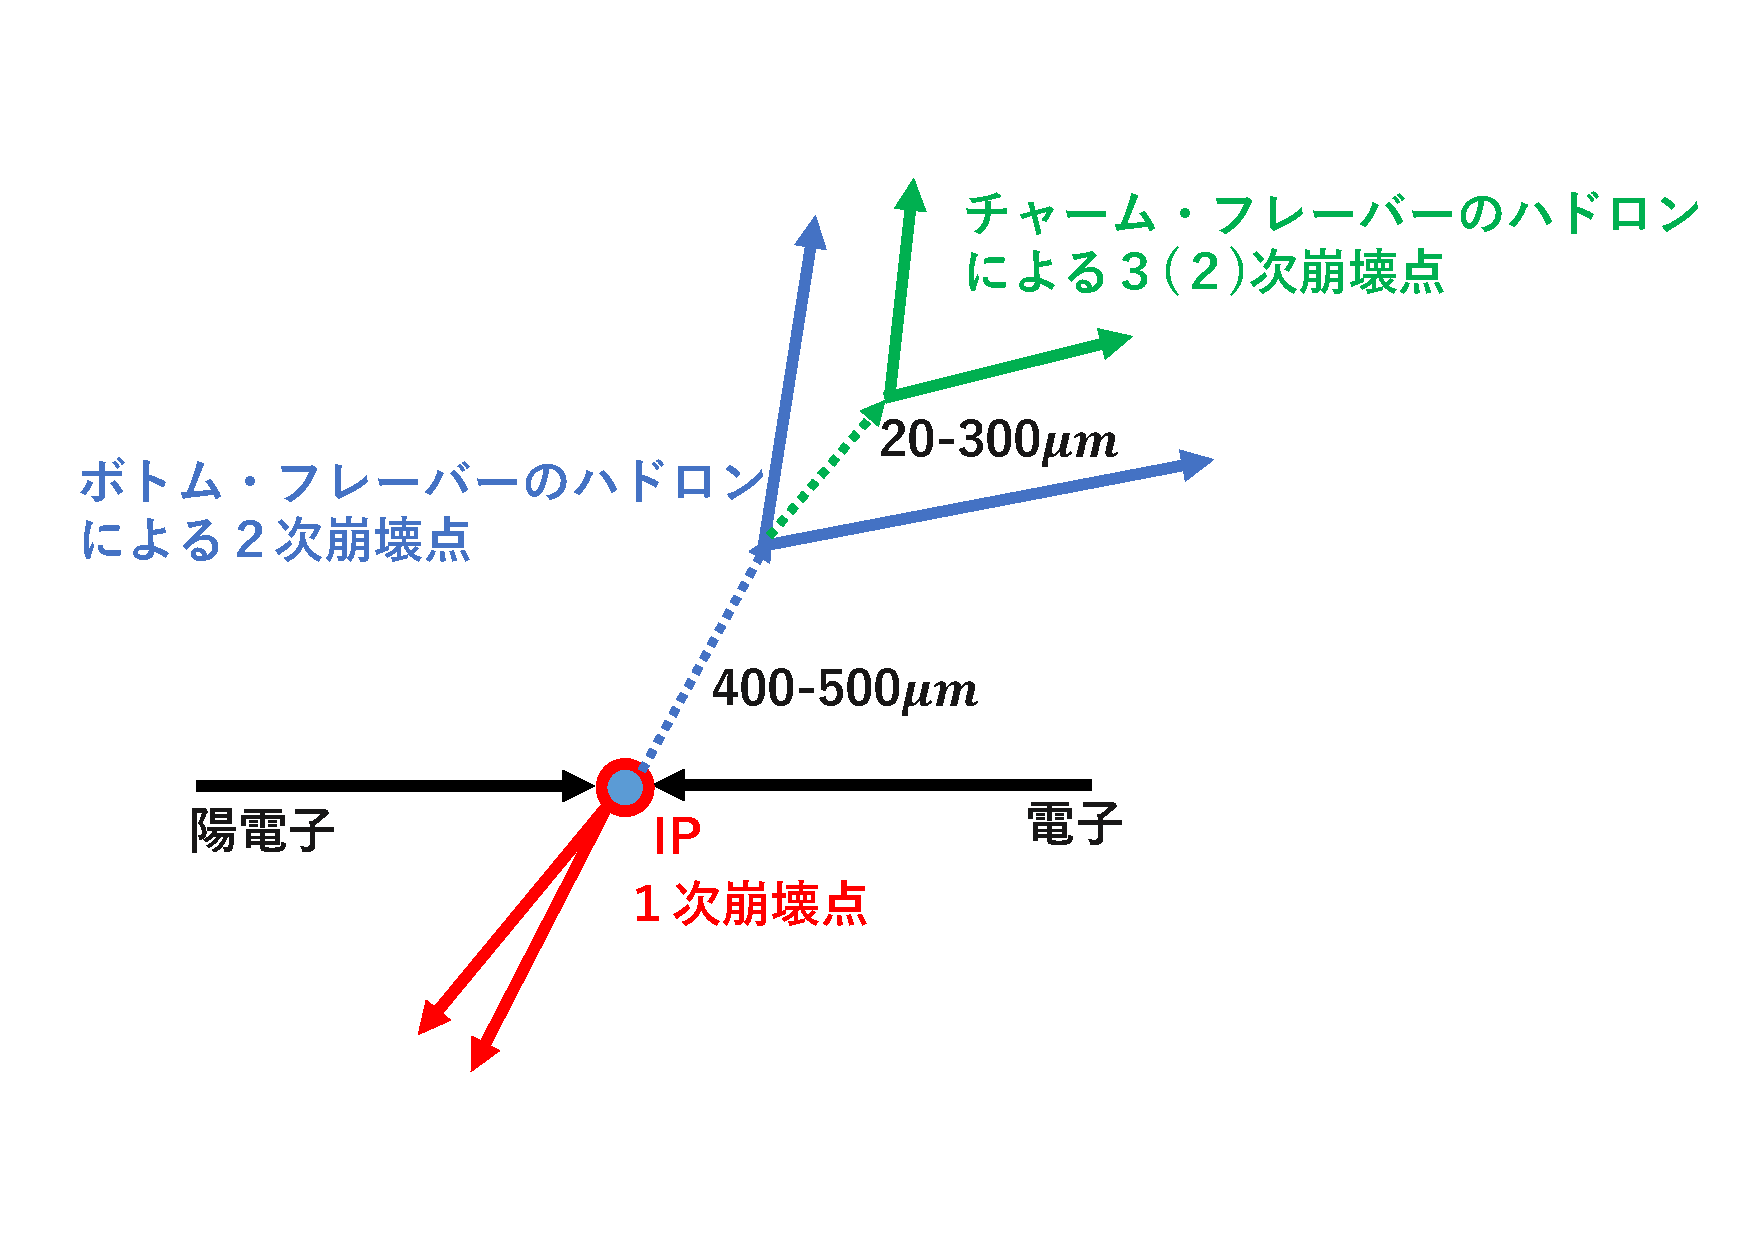
\includegraphics[keepaspectratio, scale=0.4]
 	{Figure/Introduction/bcjets.pdf}
 		\caption {ジェットの崩壊の様子。赤線が1次崩壊点、青線が2次崩壊点、緑線が3次崩壊点を由来とする飛跡を表す。}
 		\label{bcjets}
	\end{center}
\end{figure}
\section{本研究の目的}
 本研究の目的は、電子陽電子ヒッグスファクトリーであるILCにおけるジェット測定技術の開発である。ヒッグス粒子や$\SI{350}{GeV}$以上のILCで探索可能なトップクォークなど、ILCの物理において重要な事象の多くはジェットを含んでおり、ジェットを高い精度で測定することが物理解析の性能に直結する。そのジェット測定技術において、シリコンタングステン電磁カロリメータの性能評価、フレーバー識別アルゴリズムの開発の2つのテーマで研究を行った。\\
\subsection{高エネルギービームによるSiW-ECALの性能評価}
 ILCでは粒子単位での再構成が求められ、そのためにはジェットのエネルギーや方向の分解能を高い精度で得ることが重要となる。高いジェットエネルギー分解能を達成するために提案されているPFAでは、ジェット中の粒子を分離しクラスタリングが可能になるほどに高精細なカロリメータが求められており、日本やフランスのグループによって開発されたシリコンタングステン電磁カロリメータはその有望な候補である。本研究では、その技術プロトタイプに高エネルギービームを照射するビームテスト実験を行い、実験結果から更なる改善に向けたフィードバックを得た。本論文では、2章で背景となる物理やSiW-ECALの仕組みについて述べ、3章でビームテスト実験について報告する。\\
\subsection{深層学習を用いたフレーバー識別アルゴリズムの開発}
 再構成において重要なプロセスとなるフレーバー識別アルゴリズムの開発を、深層学習技術を用いて行った。本研究では、特にグラフ構造のデータを扱うグラフニューラルネットワークを実装し、従来技術であるLCFIPlusと比較した識別精度の向上を目指した。グラフニューラルネットワークでは、対象の特徴量に加え構造のトポロジー情報をデータに含んだ学習を行うことができる。また同時に、全ての事象再構成アルゴリズムを深層学習に置き換えることを最終目標に、フレーバー識別アルゴリズムと崩壊点検出アルゴリズムの統合を試みた。本論文では、4章で深層学習に関する基本的事項について述べ、5章で実際に考案したアルゴリズムについて述べる。